
\documentclass[manuscript]{aastex}
\newcommand{\myemail}{gbrunner@rice.edu}

\shorttitle{Mapping Molecular Hydrogen in NGC 5194}
\shortauthors{Brunner et al.}


\begin{document}

\title{Mapping $\mathrm{H_2}$ Excitation and Mass across M51 with the Spitzer Infrared Spectrograph}

\author{Gregory Brunner\altaffilmark{1,2}}
\affil{Department of Physics and Astronomy, Rice University, \\
    Houston, TX 77005}
\email{gbrunner@ipac.caltech.edu, gbrunner@rice.edu}

\author{Kartik Sheth\altaffilmark{3}, Lee Armus\altaffilmark{3}, and George Helou\altaffilmark{3}}
\affil{Spitzer Science Center, Pasadena, CA 91125}

\author{Eva Schinnerer\altaffilmark{4}}
\affil{Max-Planck-Intit\"{u}t f\"{u}r Astronomie, Heidelberg, Germany}

%\and 

\author{Stuart Vogel\altaffilmark{5} and Mark Wolfire\altaffilmark{5}}
\affil{Department of Astronomy, University of Maryland, College Park, MD 20741}

\and

\author{Reginald Dufour\altaffilmark{1}}
\affil{Department of Physics and Astronomy, Rice University, Houston, TX 77005}

\altaffiltext{1}{Department of Physics and Astronomy, Rice University, Houston, TX 77005}
\altaffiltext{2}{Visiting Graduate Student Fellow, Spitzer Science Center, Caltech, Pasadena, CA 91125}
\altaffiltext{3}{Spitzer Science Center, Caltech, Pasadena, CA 91125}
\altaffiltext{4}{Max-Planck-Instit\"{u}t f\"{u}r Astronomie, Heidelberg, Germany}
\altaffiltext{5}{Department of Astronomy, University of Maryland, College Park, MD 20741}


\begin{abstract}

We have mapped the $\mathrm{H_2}$ S(0) $-$ $\mathrm{H_2}$ S(5) pure rotational lines over a strip across M51 using the $Spitzer$ $Space$ $Telescope$ Infrared Spectrograph.  We find that the
% $\mathrm{H_2}$ line intensity maps reveal differences in the 
molecular gas morphology of M51 varies through each line.  We use the $\mathrm{H_2}$ maps to model the $\mathrm{H_2}$ excitation-temperature and mass across the galaxy and find that the $\mathrm{H_2}$ exists in a continuous distribution of temperatures from 100 $-$ 1000 K.  Using the low $J$ lines to trace the warm (T = 100 $-$ 300 K) $\mathrm{H_2}$, we find that the warm  $\mathrm{H_2}$ excitation-temperature is highest in the nuclear region (192 K) and lower within the spiral arms (150 $-$ 170 K).  Using the higher $J$ lines to trace the hot (T = 400 $-$ 1000 K)  $\mathrm{H_2}$, we find that the hot $\mathrm{H_2}$ excitation-temperature is lowest in the inner spiral arms (500 $-$ 550 K) and increases to $\sim$ 600 K in the nucleus, where the largest hot $\mathrm{H_2}$ mass densities are found, 0.24 $\mathrm{M_\sun}$/$\mathrm{pc^2}$.  The warm-to-hot $\mathrm{H_2}$ mass ratio is not constant across the galaxy indicating different primary excitation mechanisms for the warm and hot $\mathrm{H_2}$ phases.  We compare $\mathrm{H_2}$ to CO (J = 1 $-$ 0) emission and find offsets between the warm and hot $\mathrm{H_2}$ mass phases and the CO.
%that the $\mathrm{H_2}$ spiral arms trace the CO spiral arms, though within the spiral arms we see offsets between the peaks in $\mathrm{H_2}$ and CO intensity.  
One possible explanation for the offsets between the warm $\mathrm{H_2}$ mass and CO is that the warm $\mathrm{H_2}$ traces the sites of active star formation within the molecular clouds.  
%The offsets between the hot $\mathrm{H_2}$ mass and CO are likely due to the hot phase being excited by shocks and X-rays.  
In the nuclear region, the hot $\mathrm{H_2}$ is coincident with [O IV](25.89 $\micron$) emission and X-ray emission indicating that shocks and X-rays are the dominant excitation mechanisms of the hot $\mathrm{H_2}$ phase.
 

\end{abstract}

\keywords{galaxies: ISM --- galaxies: $\mathrm{H_2}$ --- galaxies: individual(NGC 5194)}

\section{Introduction}

Star formation and galactic evolution are linked via the molecular gas within a galaxy.  In the Milky Way, nearly all star formation occurs in molecular clouds (Blitz 1995), although not all molecular clouds are actively forming stars.  In galaxies star formation is triggered whenever the molecular gas surface density is enhanced, for example, by a spiral density wave (Vogel et al. 1988), by increased pressure or density in galactic nuclei (Young and Devereux 1991, Sheth et al. 2005),  due to the hydrodynamic shock along the leading edge of bars (Sheth et al. 2000, Sheth et al. 2002), and in the transition region at the ends of bars (Kenney and Lord 1991).  Although the connection between star formation and molecular gas is well-established, the exact mechanisms for initiating, controlling, and inhibiting star formation are not well-understood.

M51 (the Whirlpool galaxy, NGC 5194) is a nearby, face-on galaxy that is rich in molecular gas.  Its proximity (assumed to be 8.2 Mpc [Tully 1988]), orientation, and morphology make it an ideal target for studies of the ISM across distinct dynamical, chemical, and physical environments in a galaxy.  Studies of the molecular gas within M51 have revealed giant molecular associations (GMAs) along the spiral arms (Aalto et al. 1999), a reservoir of molecular gas associated with the nuclear AGN (Scoville et al. 1998), and star-formation in molecular clouds triggered by a spiral density wave (Vogel et al. 1988).  In addition to being well-studied at millimeter and radio wavelengths, M51 has been studied in X-rays, UV, optical, near-infrared, infrared,  and submillimeter wavelengths (Palumbo et al. 1985,  Terashima et al. 2001, Scoville et al. 2001, Calzetti et al. 2005, Matsushita et a. 2004).  

%Prior to the advent of space infrared observatories such as the Infrared Space Observatory (ISO) and the Spitzer Space Telescope ($Spitzer$), much of our knowledge of the conditions of the molecular hydrogen (the most abundant molecule in the interstellar medium (ISM)) in galaxies came from studies of CO emission and rotational-vibrational $\mathrm{H_2}$ line emission in the near-infrared.  CO rotational line emission traces the mass of the coldest (T = 5 $-$ 100 K) $\mathrm{H_2}$ while the near-infrared  $\mathrm{H_2}$ line emission traces the hot (T  $\geq$ 1000 K) $\mathrm{H_2}$.   

The Infrared Spectrograph (IRS) (Houck et al. 2004) on-board the $Spitzer$ $Space$ $Telescope$ is a powerful tool for observing the warm (T = 100 $-$ 300 K) and hot (T = 400 $-$ 1000 K) molecular gas within galaxies.  The $Spitzer$ IRS low resolution modules cover 5 - 38 $\micron$ (short-low, SL, 5 - 14 \micron; long-low, LL, 14 - 38 \micron) giving observers access to the lowest pure rotational $\mathrm{H_2}$ lines with the low $J$ lines tracing the warm molecular gas phase and the higher $J$ lines tracing the hot molecular gas phase.  These lines are important diagnostics of the ISM that allow us to  model the $\mathrm{H_2}$ excitation-temperature, mass (Rigopoulou et al. 2002, Higdon et al. 2006), and ortho-to-para ratio (Neufeld et al. 1998, Neufeld et al. 2006).  By understanding the pure rotational $\mathrm{H_2}$ line emission from a galaxy, constraints can be placed on the energy injection mechanisms (i.e. radiative heating, shocks, turbulence) that heat the warm molecular gas phase in the ISM.  

In this paper we present maps of the extinction-corrected $\mathrm{H_2}$ S(0) $-$ $\mathrm{H_2}$ S(5) line intensities over a strip across M51(\S3.1) and use the maps to model the warm and hot $\mathrm{H_2}$ excitation-temperature and mass across the galaxy (\S3.2 and \S3.3).  We seek to understand  whether the warm and hot phases undergo excitation via the same processes and discern the primary excitation mechanism of $\mathrm{H_2}$ across the galaxy by comparing $\mathrm{H_2}$ to CO (J = 1 $-$ 0) (\S4.1), [O IV](25.89 $\micron$) intensity (\S4.2), and X-rays (\S4.3).

\section{Observations and Data Reduction}

\subsection{Spectral Data}

We mapped a radial strip across \objectname{M51} using the short-low (SL) and long-low (LL) modules of the $Spitzer$ IRS in spectral mapping mode.  The radial strips were 324$\arcsec$ $\times$ 57$\arcsec$ and 295$\arcsec$ $\times$ 51$\arcsec$ in the SL and LL, respectively.  Integration times in the SL and LL were 14.6 s.  Each slit position was mapped twice and half-slit spacings were used.  In total, 1,412 spectra were taken in the SL and 100 were taken in the LL (including background observations).  Dedicated off source background observations were taken for the SL observations.  Backgrounds for the LL observations were taken from outrigger data collected while the spacecraft was mapping in the adjacent module.  The astronomical observation requests (AORs) are available on SST's Leopard and Spot (Project ID 200138, PI: K. Sheth).

The spectra were assembled from the basic calibration data (BCD) into spectral data cubes for each module using CUBISM (Kennicutt et al. 2003, Smith et al. 2004, Smith et al. 2007, in press).  Background subtraction and bad pixel removal was done within CUBISM.  The individual IRS spectra were processed using the S14.0 version of the Spitzer Science Center (SSC) pipeline.  In CUBISM, the SL and LL data cubes have resolutions of 1.85$\arcsec$/pixel and 5.08$\arcsec$/pixel, respectively.  The spatial resolution of the data cubes varies as a function of wavelength from 1$\farcs$85 at 5.2 $\micron$ to 13$\farcs$8 at 38 $\micron$.  %Table 1 lists the resolutions of the $\mathrm{H_2}$ line maps.

We created maps of the $\mathrm{H_2}$ S(0) $-$ $\mathrm{H_2}$ S(5) lines with PAHFIT (Smith et al. 2007), a spectral fitting routine that decomposes IRS low resolution spectra.  The advantage of using PAHFIT is that it allows the recovery of the full line flux of blended $\mathrm{H_2}$ lines such as $\mathrm{H_2}$ S(1), blended with the 17.0 $\micron$ PAH complex; $\mathrm{H_2}$ S(2), blended with [Ne II](12.8 $\micron$); and $\mathrm{H_2}$ S(5), blended into [Ar II](6.9 $\micron$).   We ran PAHFIT through the SL (SL1 + SL2) and LL (LL1+ LL2)  cubes separately.  The concatenated SL and LL data cubes were each smoothed spatially by a 3 $\times$ 3 pixel box prior to running PAHFIT to increase the signal-to-noise ratio of the spectra.  When running PAHFIT through the SL and LL data cubes we measured the extinction-corrected line intensity of every spectral line in the data cubes while saving the information about the position (RA and Dec) of each spectrum and in doing so, we constructed line-intensity maps.

\subsection{Ancillary Data: CO Map and X-ray Observations}

The BIMA (Berkely Illinois Maryland Array) CO (J = 1 - 0) map was acquired as a part of the BIMA Survey of  Nearby Galaxies (SONG) (Regan et al. 2001; Helfer et al. 2003).  The beam size is 5$\farcs$8 $\times$ 5$\farcs$1 (220 pc $\times$ 190 pc).

X-ray emission from M51 was observed by the Advanced CCD Imaging Spectrometer (ACIS) on the $Chandra$ $X$-$Ray$ $Observatory$ on 20 June 2000.  The total integration time was 14,865 seconds.  The resolution of the image is $\sim$ 1$\arcsec$.  Further details of the observations are presented in Terashima and Wilson (2001).

\section{Results}

\subsection{Morphology of $\mathrm{H_2}$ Emission}

We have detected and mapped $\mathrm{H_2}$ emission from the six lowest pure rotational lines (Figure 1).  The maps of $\mathrm{H_2}$ rotational line intensity reveal remarkable differences in the morphology of \objectname{M51} through each line.  $\mathrm{H_2}$ S(0) emission is strongest in the northwest spiral arm peaking at an intensity of 3.66 $\times$ $\mathrm{10^{-18}}$ $\mathrm{W/m^2}$ and decreases by a factor of 2 in the nuclear region.  The $\mathrm{H_2}$ S(1) emission peaks in the nucleus of the galaxy at an intensity of 1.03 $\times$ $\mathrm{10^{-17}}$ $\mathrm{W/m^2}$  and shows similar intensity moving into the northwest spiral arm.  The peaks in $\mathrm{H_2}$ S(0) and $\mathrm{H_2}$ S(1) emission within the arms are not aligned, they are offset by 10$\farcs$2 (380 pc).  These offsets are not a result of the difference in resolution between the two maps, but appear to be real. $\mathrm{H_2}$ S(0) and $\mathrm{H_2}$ S(1) emission is resolved out to 5 $-$ 6 kpc from the nucleus of the galaxy in the northwest outer spiral arm.  In the outer spiral arm, the $\mathrm{H_2}$ S(0) intensity 
is a factor of 2 times lower than in the inner northwest spiral arm and the $\mathrm{H_2}$ S(1) intensity is a factor of 5 times lower than in the nucleus of M51.
 
The $\mathrm{ H_2}$ S(2) $-$ $\mathrm{H_2}$ S(5) maps show different morphology to the molecular gas within \objectname{M51} through each $\mathrm{H_2}$ line.  The strongest $\mathrm{H_2}$ S(2) emission is from the nuclear region of \objectname{M51} peaking at 2.21 $\times$ $\mathrm{10^{-18}}$ $\mathrm{W/m^2}$.  We also see bright $\mathrm{H_2}$ S(2) emission from the inner northwest spiral arm; however, the intensity is a factor of 2 lower than in the nucleus.  The $\mathrm{H_2}$ S(3) line exhibits similar strong emission in the nuclear region.  The $\mathrm{H_2}$ S(3) intensity in the nucleus is 1.35 $\times$ $\mathrm{10^{-17}}$ $\mathrm{W/m^2}$ which is a factor of $\sim$ 6 greater than the intensity of $\mathrm{H_2}$ S(2) nuclear emission.  We see an apparent bar structure in $\mathrm{H_2}$ S(3) emission across the nucleus of the galaxy going north-to-south.  We see offsets in the intensity peaks within the spiral arms of \objectname{M51} between the $\mathrm{H_2}$ S(2) and $\mathrm{H_2}$ S(3) maps.  An example of this is in the northwest inner spiral arm of M51.  In $\mathrm{H_2}$ S(2) emission, we see bright (1.30 $\times$ $\mathrm{10^{-18}}$ $\mathrm{W/m^2}$) $\mathrm{H_2}$ emission to the north of the nucleus.  The $\mathrm{H_2}$ S(2) intensity decreases to 7.00 $\times$ $\mathrm{10^{-19}}$ $\mathrm{W/m^2}$ moving southwest in the spiral arm.  In the $\mathrm{H_2}$ S(3) emission map, we see the $\mathrm{H_2}$ S(3) intensity increasing from 4.00 $\times$ $\mathrm{10^{-18}}$ $\mathrm{W/m^2}$ to 5.10 $\times$ $\mathrm{10^{-18}}$ $\mathrm{W/m^2}$ as we move from north of the nucleus (the end of the bar structure) to the southwest in the inner spiral arm.  The offsets in the peak emission of the $\mathrm{H_2}$ lines are real and indicate variations in the excitation-temperature in each region.

The $\mathrm{H_2}$ S(4) and $\mathrm{H_2}$ S(5)  lines are faint across the disk of the galaxy but both are very strong in the nuclear region.  In the nucleus, the $\mathrm{H_2}$ S(4) intensity is 3.05 $\times$ $\mathrm{10^{-18}}$ $\mathrm{W/m^2}$ and the $\mathrm{H_2}$ S(5) intensity is 8.04 $\times$ $\mathrm{10^{-18}}$ $\mathrm{W/m^2}$.  $\mathrm{H_2}$ S(5) emission is asymmetric in the nucleus and mimics the morphology of the $\mathrm{H_2}$ S(3) line with extended emission to the north of the nucleus.  The $\mathrm{H_2}$ S(4) line shows emission in the nucleus and in the spiral arm to the west.  In the spiral arm to the west of the nucleus, the $\mathrm{H_2}$ S(4) intensity is 2.11 $\times$ $\mathrm{10^{-18}}$ $\mathrm{W/m^2}$.  This is notable because the spiral arm to the southwest of the nucleus is very bright in CO and and studies have revealed very high molecular gas column densities in the southwest inner spiral arm (Lord and Young 1990).  The differences in the morphology of $\mathrm{H_2}$ emission are indicative of changes in the $\mathrm{H_2}$ excitation-temperature across the galaxy, which we discuss in the next section.

\subsection{Mapping $\mathrm{H_2}$ Excitation-Temperature and Mass across M51}

\subsubsection{Modeling $\mathrm{H_2}$ Excitation-Temperature and Mass}

The pure rotational lines of molecular hydrogen provide a powerful probe of the conditions of the ISM and place constraints on the energy injection processes that excite $\mathrm{H_2}$ (Neufeld et al. 2006).  From the maps of $\mathrm{H_2}$ S(0) $-$ $\mathrm{H_2}$ S(5) emission, we have modeled the $\mathrm{H_2}$ excitation-temperature and mass (Rigopoulou et al. 2002, Higdon et al. 2006) across M51. 

In order to model the $\mathrm{H_2}$ excitation and mass across the galaxy, the $\mathrm{H_2}$ S(1) $-$ $\mathrm{H_2}$ S(5) maps were smoothed to the resolution of the $\mathrm{H_2}$ S(0) map.
%, 10$\farcs$2 (380 pc).  
The maps were then interpolated to the same spatial grid.  Excitation diagrams across the strip were derived from the Boltzman equation using the formulation from Rigopoulou et al. (2002),
\begin{equation}
N_i/N = (g(i)/Z(\mathrm{T_{ex}}))exp(-T_i/\mathrm{T_{ex}})
\end{equation}
where $g(i)$ is the statistical weight of state $i$, Z($\mathrm{T_{ex}}$) is the partition function, $\mathrm{T_i}$ is the energy level of a given state, and $\mathrm{T_{ex}}$ is the excitation temperature.  N and $\mathrm{N_i}$ are the total column density and the column density of a given state $i$ and $\mathrm{N_i}$ is determined directly from the measured extinction-corrected flux by
\begin{equation}
N_i = 4 \pi \times flux(i)/(\Omega A(i)h\nu (i))
\end{equation}
where A($i$) is the $A$-coefficient,  $\nu$($i$) is the frequency of state $i$, $\Omega$ is the solid angle of the beam, and $h$ is Planck's constant.  Table 1 lists the values for the wavelength, rotational state, Einstein $A$-coefficient, energy, and statistical weight of the pure rotational levels of $\mathrm{H_2}$ that we have observed with the $Spitzer$ IRS. 

In Figure 2, we present excitation diagrams from three different regions across the M51 strip.  The excitation diagrams exhibit an ortho-to-para ratio (OPR) of 3 in the nuclear region.  This is in agreement with the value of the OPR of the nuclear region determined by SINGS (Roussel et al. 2007, in press).  Outside the nucleus, the lower $J$ ($\mathrm{H_2}$ S(0) - $\mathrm{H_2}$ S(3)) levels exhibit an OPR of 3.  The $\mathrm{H_2}$ S(4) measurement shows significant scatter in the excitation diagrams outside of the nuclear region of M51.   This would indicated that the OPR is less than 3; however, due to the low signal-to-noise ratio of the $\mathrm{H_2}$ S(4) map, we do not believe that the OPR determined from the $\mathrm{H_2}$ S(4) intensity reflects the OPR of the warm $\mathrm{H_2}$.  The excitation-diagrams also exhibit a change in slope as a function of rotational level.  This indicates that a continuous distribution of $\mathrm{H_2}$ temperatures is being sampled within the beam.

Because the excitation diagrams (shown in Figure 2) indicate that we are sampling a range of excitation-temperatures in different regions across the M51 strip, we assume that the $\mathrm{H_2}$ exists in the form of two discrete components.  We define these two components as a warm (T = 100 $-$ 300 K) $\mathrm{H_2}$ phase and a hot (T = 400 $-$ 1000 K) $\mathrm{H_2}$ phase.  We determine the excitation-temperature and mass distribution of the hot  (T= 400 $-$ 1000 K) $\mathrm{H_2}$ phase from the least squares fit to the $\mathrm{H_2}$ S(2) $-$ $\mathrm{H_2}$ S(5) lines in the excitation diagram.  We determine the excitation-temperature and mass distribution of the warm (T = 100 $-$ 300 K) $\mathrm{H_2}$ phase from the least squares fit to the $\mathrm{H_2}$ S(0) $-$ $\mathrm{H_2}$ S(2) lines in the excitation diagram; however, because the warm and hot $\mathrm{H_2}$ phases are inherently coupled, we subtract the the contribution of the hot $\mathrm{H_2}$ from the warm $\mathrm{H_2}$ in order to determine the warm $\mathrm{H_2}$ excitation-temperature and mass (Higdon et al. 2006).

\subsubsection{Warm and Hot $\mathrm{H_2}$ Mass Distributions}

In Figure 3 we present the warm ($left$) and hot ($right$) $\mathrm{H_2}$ mass distributions across the M51 strip.  Note that the non-rectangular shape of the strip is due to the offset between the SL and LL strips.  Also note that the sizes of the plots of the warm and hot $\mathrm{H_2}$ mass phases are different.  The warm $\mathrm{H_2}$ mass is determined from the $\mathrm{H_2}$ S(0) $-$ $\mathrm{H_2}$ S(2) maps which show $\mathrm{H_2}$ emission across the entire strip.  The hot $\mathrm{H_2}$ mass is determined from the higher $J$ rotational states from which the $\mathrm{H_2}$ emission is not well-resolved across the entire strip.  The warm $\mathrm{H_2}$ mass peaks in the inner northwest spiral arm with 11 $\mathrm{M_\sun}$/$\mathrm{pc^2}$ warm $\mathrm{H_2}$. The mass in the outer northwest and southeast spiral arms 
%(at 5 - 6 kpc from the center of the galaxy each) 
peaks toward the center of the spiral arms with 3.5 $\mathrm{M_\sun}$/$\mathrm{pc^2}$ warm $\mathrm{H_2}$ and 1.0 $\mathrm{M_\sun}$/$\mathrm{pc^2}$ warm $\mathrm{H_2}$ (in the northwest and southeast arms, respectively).

The peak in hot $\mathrm{H_2}$ mass is bimodal with a peak in the nucleus of the galaxy containing 0.24 $\mathrm{M_\sun}$/$\mathrm{pc^2}$ and a second peak that is interior to the inner spiral arm, also containing 0.24 $\mathrm{M_\sun}$/$\mathrm{pc^2}$.  The hot $\mathrm{H_2}$ mass in the spiral arms is only $\sim$ 20 - 30 \% of the hot $\mathrm{H_2}$ mass in the nucleus.
We would like to note that in M51, 
%within a 10$\farcs$2 beam, 
we are sensitive to 
%$\sim$ 5.75 $\times$ $\mathrm{10^4}$  $\mathrm{M_\sun}$ warm $\mathrm{H_2}$ and 7.75 $\times$ $\mathrm{10^2}$  $\mathrm{M_\sun}$ hot $\mathrm{H_2}$ 
0.40 $\mathrm{M_\sun}$/$\mathrm{pc^2}$ warm $\mathrm{H_2}$ and 0.005 $\mathrm{M_\sun}$/$\mathrm{pc^2}$ hot $\mathrm{H_2}$ within our beam.

\subsubsection{Warm and Hot $\mathrm{H_2}$ Excitation-Temperature Distributions}

In Figure 4, we compare the warm $\mathrm{H_2}$ mass distribution to the excitation-temperature.  The gas is warmest in the nuclear region of \objectname{M51} with the temperature ranging from 175 $-$ 190 K in the center of the galaxy.  The gas is cooler within the spiral arms of \objectname{M51} than in the inter-arm regions.  The temperature in this spiral arm decreases from 175 K at the outer surface layers to 154 K in the most dense region of the arm indicating that the warm $\mathrm{H_2}$ excitation-temperature is cooler at higher $\mathrm{H_2}$ densities.  In the outer northwest and southeast spiral arms (at 5 - 6 kpc from the center of the galaxy each) molecular the gas excitation-temperature ranges from 150 K at the center to about 175 K near the edge of the spiral arms again indicating that high density regions are cooler than low density regions.  

The excitation-temperature distribution of the hot $\mathrm{H_2}$ (in Figure 5) reveals a different picture than the excitation-temperature distribution of the warm $\mathrm{H_2}$.  The excitation-temperature in the nuclear region ranges from 587 to 612 K.  The excitation-temperature in the northwest inner spiral arm is the coldest at 538 K.  The hottest excitation-temperatures are observed in the inter-arm regions, where there is the least amount of $\mathrm{H_2}$.  In the southeast inter-arm region, the excitation temperature is in excess of 900 K.

\section{Discussion}

\subsection{Comparison to Previous Studies of $\mathrm{H_2}$ in Galaxies}

Previous studies of pure rotational $\mathrm{H_2}$ emission in galaxies have used aperture average spectra over the central regions of galaxies to derive the excitation temperature and mass of the warm and hot molecular gas phases within a galaxy (Rigopoulou et al. 2002, Higdon et al. 2006, Roussel et al. 2007, in press).  The $Spitzer$ $Infrared$ $Nearby$ $Galaxies$ $Survey$ (SINGS) has studied molecular hydrogen in M51 and finds that within the central 330 $\mathrm{arcsec^2}$, the excitation-temperature and mass of the warm (T = 100 $-$ 300 K) $\mathrm{H_2}$ phase are T = 180 K and $\mathrm{M_{warm}}$ = 1.46 $\times$ $\mathrm{10^6}$ $\mathrm{M_\sun}$, respectively (Roussel et al., in press).  Within the central 
%20$\farcs$32 $\times$ 20$\farcs$32 (
412 $\mathrm{arcsec^2}$ of M51, we measure a warm $\mathrm{H_2}$ excitation-temperature of 186 K and mass of 1.63 $\times$ $\mathrm{10^6}$ $\mathrm{M_\sun}$, consistant with the SINGS to within 10 \%.  SINGS also measures the excitation-temperature of the hot phase (though they do not measure the mass in the hot phase) and find a hot $\mathrm{H_2}$ excitation-temperature of 521 K.  Over the nuclear region of M51, we measure an excitation-temperature of 584 K.  

Rigopoulou et al. (2002) measures the $\mathrm{H_2}$ mass in the hot phase and finds that the warm-to-hot mass fraction varies between 5 $\times$ $\mathrm{10^3}$ $-$ 1 $\times$ $\mathrm{10^6}$ for Seyferts.  This is significantly higher than the warm-to-hot mass fraction (Figure 6) than we measure within the central 412 $\mathrm{arcsec^2}$ of NGC 5194, 14.8.  To measure the hot $\mathrm{H_2}$ mass, we use the $\mathrm{H_2}$ S(2) $-$ $\mathrm{H_2}$ S(5) lines, whereas Rigopoulou et al. (2002) uses the $\mathrm{H_2}$ S(5) $-$ $\mathrm{H_2}$ S(7) lines.  Thus, the hot $\mathrm{H_2}$ phase that they measure is preferentially offset to higher $\mathrm{H_2}$ excitation-temperatures and lower $\mathrm{H_2}$ masses.  


%(though the sensitivity to the hot $\mathrm{H_2}$ could be underestimated due to smoothing the $\mathrm{H_2}$ S(2), $\mathrm{H_2}$ S(3), $\mathrm{H_2}$ S(4), and $\mathrm{H_2}$ S(5) lines by a factor of 2 - 4 times their resolution).

\subsection{The Warm-to-Hot $\mathrm{H_2}$ Mass Ratio}

In Figure 6, we compare the warm $\mathrm{H_2}$ mass distribution to the hot $\mathrm{H_2}$ mass distribution.  The warm $\mathrm{H_2}$ mass distribution peaks at 
in the northwest inner spiral arm and the hot $\mathrm{H_2}$ mass distribution peaks at
in the nucleus and in the region interior to the northwest spiral arm.  It is evident from Figure 6 that the warm-to-hot $\mathrm{H_2}$ mass ratio is not constant across the galaxy.  The warm-to-hot $\mathrm{H_2}$ mass ratio is lowest in the nucleus of the galaxy at 12 and increases to 170 and 136 in the southeast and northwest spiral arms, respectively.  The differences between the warm and hot $\mathrm{H_2}$ mass distributions and the variations in the morphology of M51 as a  function of rotational energy level suggest different origins to the warm and hot $\mathrm{H_2}$ phases and that the primary excitation mechanisms of the warm and hot $\mathrm{H_2}$ phases differ.  
 
In order to understand the $\mathrm{H_2}$ excitation and where each excitation mechanism is dominant, we present comparisons of the $\mathrm{H_2}$ line intensity and mass distributions to diagnostics of three excitation mechanisms: UV photons emitted in dense photon dominated regions (PDRs), shocks, and X-rays.  We use CO (J = 1 $-$ 0) emission as to determine the location of the $\mathrm{H_2}$ mass to locations dense PDRs, [O IV](25.98 $\micron$) line emission as a diagnostic of shocks (Schaerer and Stasinska 1999), and the 0.5 $-$ 10.0 keV X-ray band to distinguish X-ray dominated regions (XDRs).  The following section compares the $\mathrm{H_2}$ mass distributions to CO (J = 1 - 0), [O IV](25.89 $\micron$), and X-ray emission.

\subsection{Distinguishing the $\mathrm{H_2}$ Excitation Mechanisms}

\subsubsection{$\mathrm{H_2}$ Excitation in PDRs: Comparison of $\mathrm{H_2}$ to CO emission}

In star-forming regions, $\mathrm{H_2}$ exists within the PDR and deep into the molecular cloud.  Owing to an ionization potential of 4.5 eV, $\mathrm{H_2}$ formation generally does not occur within a PDR until the radiation field  becomes sufficiently weak.  Understanding $\mathrm{H_2}$ in PDRs and implementing $\mathrm{H_2}$ into photoionization codes has become the emphasis of many theoretical models.  Recent advances in the CLOUDY photoionization code have included $\mathrm{H_2}$ and modeled the structure of star-forming regions while treating the HII region and PDR as one continuous cloud (Shaw et al. 2005, Abel et al. 2005).  Kaufman et al. (2006) used Starburst99/Mappings to model $\mathrm{H_2}$ pure rotational line emission from PDRs to probe the conditions of dense PDRs in star-forming regions.  They show that within galaxies, where the telescope beam size is generally kiloparsecs across, $\mathrm{H_2}$ emission could serve to probe the surface layers of dense molecular clouds.

CO is found deep within a molecular cloud where the temperatures are too cold to excite $\mathrm{H_2}$ emission.  In these regions, CO is collisionally excited by the more abundant $\mathrm{H_2}$ molecule.  CO is connected to $\mathrm{H_2}$ in star-forming regions because at the surface layers of the molecular clouds, $\mathrm{H_2}$ is excited and CO emits dipole rotational lines due to heating by the ionizing radiation of newborn massive stars (Allen et al. 2004). 
%Thus, molecular gas within molecular clouds has generally been studied via observations of CO rotational line emission.  Here, we compare the warm and hot $\mathrm{H_2}$ mass phases and $\mathrm{H_2}$ rotational line emission to CO (J = 1 - 0) emission (mapped  by BIMA SONG) in order to understand the relationship between $\mathrm{H_2}$ emission and PDRs.

In Figure 7, we compare the warm ($left$) and hot $\mathrm{H_2}$ ($right$) mass distributions to CO (J=1 - 0) emission.  The brightest CO emission is seen in the spiral arms where the greatest amounts of warm $\mathrm{H_2}$ mass are also found.  The most striking result is that in the inner spiral arms, we see that the CO is offset toward the nucleus from the warm $\mathrm{H_2}$ mass.  The offset between the peaks in CO and warm $\mathrm{H_2}$ mass is 7$\farcs$2 in the northwest spiral arms and 5$\arcsec$ in the southeast spiral arms.  We believe that these offsets are real and are not due to pixel size of the LL data cubes with one possible explanation being that the $\mathrm{H_2}$ is tracing the regions of active star-formation within the giant molecular associations.

We compare CO to the hot $\mathrm{H_2}$ mass distribution (Figure 7, $right$) and we see that the hot $\mathrm{H_2}$ mass is most abundant in the nuclear region, interior to the CO bright spiral arms.  In northwest spiral arm, the hot $\mathrm{H_2}$ mass is offset from the CO by 2$\farcs$6. We believe that the offsets between the CO  and the hot $\mathrm{H_2}$ mass are real, however, they are likely due to the dominance of other excitation mechanisms (shocks or X-rays) in the nuclear region of M51.

%Within the spiral arms, the $\mathrm{H_2}$ mass is generally aligned with CO emission; however, there are offsets in the location of the peaks in the $\mathrm{H_2}$ mass and CO emission.  This is real and is not due to the difference in resolution between the CO map (6$\arcsec$) and the $\mathrm{H_2}$ maps (10$\farcs$2).  In the northwest inner spiral arm, the peak in warm $\mathrm{H_2}$ mass is offset to the northwest of the peak in CO emission.  At even larger distances from the nucleus of NGC 5194, we observe the $\mathrm{H_2}$ mass offset from the CO emission within the outer northwest spiral arm.  In this case, the $\mathrm{H_2}$ mass is offset to the southeast of the CO emission.  Additionally, in the southeast outer spiral arm we observe $\mathrm{H_2}$ in a region that appears devoid of CO emission.  These regions, where the peaks are offset or there is no CO emission where $\mathrm{H_2}$ is observed could just be spiral arms that are rich in $\mathrm{H_2}$ but devoid of CO.   Comparing the hot $\mathrm{H_2}$ mass phase to CO emission (Figure 7, $right$), the hot $\mathrm{H_2}$ mass peaks in the nucleus and in the region interior to the CO spiral arm.  In the  northwest and southeast spiral arms, CO emission is found within the wider $\mathrm{H_2}$ mass contours. This is a result of the difference in resolution between the $\mathrm{H_2}$ maps and the BIMA SONG CO map.   

In Figure 8, we compare the CO intensity to the $\mathrm{H_2}$ S(0) - $\mathrm{H_2}$ S(3) line intensity maps.  We see that the $\mathrm{H_2}$ S(0) contours trace the CO spiral arms with one notable difference being that we detect $\mathrm{H_2}$ S(0) emission far (5 $-$ 6 kpc) from the nucleus of M51, where there is no CO detected.  The $\mathrm{H_2}$ S(1) $-$ $\mathrm{H_2}$ S(3) contours also trace the CO spiral arms; however, within the spiral arms, the $\mathrm{H_2}$ is not necessarily aligned with the CO.  For example, in the comparison of $\mathrm{H_2}$ S(3) to CO, we see that in the inner spiral arms, the $\mathrm{H_2}$ contours trace the CO; however, within the northwest arm, we see that there is strong $\mathrm{H_2}$ emission offset to the west by 9$\farcs$ from the bright CO emission in the same spiral arm.  The offsets between the peaks in $\mathrm{H_2}$ and CO emission are not systematic in any direction.

The CO intensity in the nucleus of the galaxy is much fainter than in the bright CO spiral arms.  This is interesting because $\mathrm{H_2}$ S(1) $-$ $\mathrm{H_2}$ S(3) emission is brightest in the nucleus of M51 where $\mathrm{H_2}$ emission from the higher $J$ lines is likely due to more energetic processes such as shock excitation and X-rays (which we explore in the next subsection).

%These maps all resolve $\mathrm{H_2}$ emission within the nucleus and spiral arms of the galaxy.  The $\mathrm{H_2}$ S(2) and $\mathrm{H_2}$ S(3) maps (at resolutions of  3$\farcs$44 and 4$\farcs$37, respectively) show strong correlation between $\mathrm{H_2}$ and CO emission within the spiral arms.   In the spiral arms, the $\mathrm{H_2}$ emission generally traces the CO emission with the one exception that in the $\mathrm{H_2}$ S(2) map, $\mathrm{H_2}$ emission in the southeast spiral arm is offset to the southeast by 2$\arcsec$ from the CO spiral arm.  Comparing the $\mathrm{H_2}$ S(1) map to CO emission shows that a strong correlation between $\mathrm{H_2}$ and CO  emission in the spiral arms.  In this case both maps are at similar resolutions ( $\sim$ 6$\arcsec$) and the $\mathrm{H_2}$ contours trace the CO emission (though it should be noted that the $\mathrm{H_2}$ contours appear wider than the CO emission; this is an effect of grouping spectra prior to fitting).  The comparison between the $\mathrm{H_2}$ S(0) and CO emission shows that the $\mathrm{H_2}$ S(0) and CO emission are correlated; however, we notice offsets in the emission peaks for CO and $\mathrm{H_2}$ S(0).  While we notice offsets between the $\mathrm{H_2}$ S(0) and CO emission peaks, a correlation between $\mathrm{H_2}$ and CO emission in the spiral arms is evident.  In general, the $\mathrm{H_2}$ emission traces the CO spiral arms and except for in the southwest spiral arm, the $\mathrm{H_2}$ S(2) and $\mathrm{H_2}$ S(3) emission from the spiral arms is co-spatial with the CO emission.  This suggests that the $\mathrm{H_2}$ emission in the spiral arms is associated with the surface layers of PDRs, as predicted by Kaufman et al. (2006).

%While $\mathrm{H_2}$ rotational line emission and CO are correlated in the spiral arms, the peaks in $\mathrm{H_2}$ S(2) and $\mathrm{H_2}$ S(3) intensity both occur in the nucleus of NGC 5194.  Within the $\mathrm{H_2}$ S(2) and $\mathrm{H_2}$ S(3) emission peaks, faint CO emission is offset to the north of the $\mathrm{H_2}$ intensity peaks.  This suggests that while $\mathrm{H_2}$ emission is excited within PDRs associated with dense molecular clouds in the spiral arms, a different process is the dominant excitation mechanism of the higher $J$ lines and the hot $\mathrm{H_2}$ phase within the nuclear region of NGC 5194.

\subsubsection{$\mathrm{H_2}$ Excitation by Shocks: Comparison of $\mathrm{H_2}$ to [OIV](25.89 \micron) emission}

The [O IV](25.89 \micron) line can be excited in shocks (Schaerer and Stasinska 1999), the stellar winds of massive Wolf-Rayet stars (Lutz et al. 1998), or by an active galactic nucleus (AGN)(Smtih et al. 2004).  Though the [O IV](25.89 \micron) line is bleneded with the [Fe II](25.99 \micron) line in $Spitzer$ IRS low resolution spectra, PAHFIT can deblend the two lines and in mapping the $\mathrm{H_2}$ S(0) and $\mathrm{H_2}$ S(1) line in the LL data cubes, we also mapped the [O IV](25.89 \micron) line.
%emission was also be mapped at a resolution of 9$\farcs$39 ($\lambda$/$\delta$$\lambda$ = 142). 

In figure 9, we compare the [O IV](25.89 \micron) intensity to the warm and hot $\mathrm{H_2}$ disributions.  
%The [O IV](25.89 \micron) line intensity map, warm $\mathrm{H_2}$ map, and hot $\mathrm{H_2}$ map all have comparable resolutions (9$\farcs$39, 10$\farcs$2, and 10$\farcs$2, respectively).  
The [O IV](25.89 $\micron$) emission is brightest in the nuclear region at 8.75 $\times$ $\mathrm{10^{-18}}$ $\mathrm{W/m^2}$ and the peak is coincident with the nuclear peak in the mass of the hot $\mathrm{H_2}$.  [O IV](25.89 $\micron$) emission subsides from the nucleus to the inner spiral arm by 50 \%.  We resolve weaker [O IV](25.89 $\micron$) emission within the warm and hot $\mathrm{H_2}$ spiral arms.  The  [O IV](25.89 $\micron$) intensity in the spiral arms is a factor of $\sim$ 6 lower in the spiral arms than the peak intensity found in the nucleus.

The [O IV](25.89 $\micron$) emission within the nuclear region is likely due to the weak Seyfert II nucleus (Ford et al. 1985) and is possibly associated with shocked gas from the outflows of the AGN.  The peak of the [O IV](25.89 $\micron$) emission coincides with the nuclear peak in hot $\mathrm{H_2}$ mass indicating that the hot $\mathrm{H_2}$ phase in the nuclear region of the galaxy is AGN or shock heated.  With 2.43 $\times$ $\mathrm{10^5}$ $\mathrm{M_\sun}$ of hot $\mathrm{H_2}$ in the central 0.58 $\mathrm{kpc^2}$, it is unlikely that the hot $\mathrm{H_2}$ is fueling the central AGN, but is excited by the AGN or shocks produced by it.  In the nuclear region we observe a factor of 12 times greater warm $\mathrm{H_2}$ mass.  The warm $\mathrm{H_2}$ mass is much greater within the spiral arms than within the nucleus and the warm-to-hot mass ratio is lowest in the nuclear region where the  [O IV](25.89 \micron) intensity is greatest.  In the nuclear region, shocks appear to be a more efficient means to excite the hot $\mathrm{H_2}$ phase than the warm $\mathrm{H_2}$ phase.

% the warm $\mathrm{H_2}$ is not primarily excited by shocks.

\subsubsection{$\mathrm{H_2}$ Excitation by XDRs: Comparison of $\mathrm{H_2}$ to X-ray emission}

M51 has been extensively studied in X-rays by ASCA (Terashima et al. 1998), Newton XMM (Dewangen et al. 2005), and  the Chandra X-ray Observatory (Terashima and Wilson 2001). These observations of M51 have revealed more than 80 X-ray sources.  Candidates for these X-ray sources include neutron stars, black holes, supernova remnants (SN 1994I), and a low-luminosity AGN (Terashima et al. 2006, Immler et al. 2002, Terashima and Wilson 2001).  X-ray emission from the nuclear region of M51 has been studied by Terashima and Wilson (2001).  They observe X-ray emission from the nucleus, the extranuclear cloud (XNC, to the south of the nucleus), and the northern loop.  A radio jet has been observed connecting the nucleus of NGC 5194 to the XNC in 6 cm imagery (Crane and van der Hulst 1992).  The jet emanates from the south of the elongated nucleus and is shock heating ISM.

In figure 10 we compare the smoothed 0.5 - 10 keV band X-ray image to the warm ($left$) and hot ($right$) $\mathrm{H_2}$ mass distributions.  The 0.5 - 10 keV band has been smoothed to the resolution of the warm and hot $\mathrm{H_2}$ mass distributions and the nucleus, XNC, and northern loop are indistinguishable in the smoothed image.  X-ray emission is most intense from the nucleus and decreases into the northwest spiral arm that contains the greatest $\mathrm{H_2}$ mass and there appears to be very little connection between the 0.5 - 10 keV X-ray band and the warm $\mathrm{H_2}$ mass distribution.  

The peak in X-ray emission is coincident with the hot $\mathrm{H_2}$ mass peak. The most intense 0.5 - 10 keV X-ray emission originates from the nucleus and is oriented north-to-south, similar to the [O IV](25.89 $\micron$) emission.
The peak in X-ray emission is located within the peak in hot $\mathrm{H_2}$ mass suggesting that X-rays play an important role in exciting the hot $\mathrm{H_2}$ phase.  While there is a correlation between X-ray emission and the hot $\mathrm{H_2}$ phase, $\mathrm{H_2}$ excitation by X-rays cannot be distinguished from $\mathrm{H_2}$ excitation by shocks.  

%When smoothed to 10$\farcs$2 resolution, the X-ray distribution mimics the [O IV](25.89 $\micron$) emission map.

%; however, due to the disparity in resolution between the X-ray image and the $\mathrm{H_2}$ maps (1$\arcsec$ resolution for X-rays, 10$\farcs$2 resolution for the warm and hot $\mathrm{H_2}$ mass) it is difficult to distinguish between shock excitation and X-ray excitation of $\mathrm{H_2}$ in the nuclear region of NGC 5194.  

We further investigate X-ray excited $\mathrm{H_2}$ emission in M51 by comparing the 0.5 $-$ 10.0 keV X-ray band to the $\mathrm{H_2}$ S(2) $-$ $\mathrm{H_2}$ S(5) line intensity maps (Figure 11).   The $\mathrm{H_2}$ S(2), $\mathrm{H_2}$ S(3), $\mathrm{H_2}$ S(4), and $\mathrm{H_2}$ S(5) line intensities all peak at the X-ray source within the nucleus.  The X-ray source fits within the $\mathrm{H_2}$ contours because the X-ray image resolution is slightly higher than the resolution of each of the $\mathrm{H_2}$ maps.  

The morphology of the nuclear $\mathrm{H_2}$ emission appears to be correlated with the X-ray source.  The $\mathrm{H_2}$ S(2) intensity peaks around the X-ray nucleus and the intensity decreases to the south by 70 \% in the southern XNC.  The bar structure seen in the $\mathrm{H_2}$ S(3) emission is aligned with X-ray emission from the nucleus, XNC, and northern loop.  The $\mathrm{H_2}$ S(3) intensity peaks between the X-ray nucleus and the XNC.  To the north of the nucleus, the contours follow the X-ray loop.  To the south of the nucleus (into the XNC), $\mathrm{H_2}$ S(3) intensity decreases by 80 \%.  The $\mathrm{H_2}$ S(4) and $\mathrm{H_2}$ S(5) line intensities are highest in the nucleus which coincides with strong X-ray emission from the nucleus and XNC.

\section{Conclusions}

We have spectrally mapped a strip across M51 using the $Spitzer$ IRS low resolution modules.  We used the spatially resolved spectra to map $\mathrm{H_2}$ S(0) $-$ $\mathrm{H_2}$ S(5) line intensities across the strip.  We find:\\
\\
1.  The morphology of $\mathrm{H_2}$ emission in M51 varies with $\mathrm{H_2}$ rotational level.  $\mathrm{H_2}$ S(0) emission is strongest in the spiral arms of the galaxy while the higher $J$ transitions show the strongest emission towards the nucleus.  The $\mathrm{H_2}$ S(1) intensity is strongest in the nuclear region and in the northwest spiral arms, however, the peak in $\mathrm{H_2}$ intensity in the northwest spiral arm is offset from the peak in $\mathrm{H_2}$ S(0) intesity by 10$\farcs$2.  The $\mathrm{H_2}$ S(2) and $\mathrm{H_2}$ S(3) maps show $\mathrm{H_2}$ emission in the nucleus, spiral arms, and inter-arm regions of M51 and bar structure aligned north-to-south is apparent in $\mathrm{H_2}$ S(3) emission.  $\mathrm{H_2}$ S(4) and $\mathrm{H_2}$ S(5) emission is resolved in the nuclear region of M51.\\  
%The $\mathrm{H_2}$ S(5) morphology mimics the $\mathrm{H_2}$ S(3) morphology and the $\mathrm{H_2}$ S(4) morphology shows 
%maps reveal interesting morphology to the molecular gas distributions, such as bar structure across the nucleus in $\mathrm{H_2}$ S(3) emission.\\
\\
2.  The different morphologies of  $\mathrm{H_2}$ emission in M51 indicate variations in $\mathrm{H_2}$ excitation-temperature and mass.  
Excitation diagrams reveal that the $\mathrm{H_2}$ exists in a continuous distribution of temperatures across the galaxy.  
Using the low $J$ lines to trace the warm (T = 100 $-$ 300 K) $\mathrm{H_2}$, we find that the warm  $\mathrm{H_2}$ excitation-temperature is highest in the nuclear region at 192 K and the warm $\mathrm{H_2}$ mass peaks in the northwest inner spiral arm at a mass density of 11 $\mathrm{M_\sun}$/$\mathrm{pc^2}$.  Using the higher $J$ lines to trace the hot (T = 400 $-$ 1000 K)  $\mathrm{H_2}$, we find that the hot $\mathrm{H_2}$ excitation-temperature is lowest in the inner spiral arms (500 $-$ 550 K) and increases to $\sim$ 600 K in the nucleus, where the largest hot $\mathrm{H_2}$ mass densities are found, 0.24 $\mathrm{M_\sun}$/$\mathrm{pc^2}$.\\
%We assume that the $\mathrm{H_2}$ exists in the form of two phases, a warm (T = 100 - 300 K) phase and a hot (T = 400 - 1000 K) phase.  
\\
3.  The warm and the hot $\mathrm{H_2}$ mass are not cospatial and the warm-to-hot mass ratio varies across M51.  The hot mass distribution shows two peaks, one in the nucleus of M51 and one located interior to the northwest inner spiral arm of M51.  The warm mass distribution peaks in the northwest spiral arm and is offset from the hot mass peak by 11$\farcs$4.  The warm-to-hot mass ratio varies across the galaxy with the ratio being $\sim$ 15 in the nucleus and increasing to $\geqq$ 100 in the spiral arms.  Variations in the warm-to-hot $\mathrm{H_2}$ mass ratio and differences in the morphology of the $\mathrm{H_2}$ emission across M51 indicate that the primary excitation mechanism differs for the warm and hot $\mathrm{H_2}$ mass phases as a function of location within the galaxy.\\
\\
4. CO emission is offset from the warm $\mathrm{H_2}$ mass in the inner spiral arms of M51.  These apparent offsets are real and are possibly associated with the regions of active star formation within the molecular clouds.  In the spiral arms, the $\mathrm{H_2}$ S(0) $-$ $\mathrm{H_2}$ S(3) contours trace the CO; however, within the spiral arms, the peaks in $\mathrm{H_2}$ can be offset from the peaks in CO intensity.  In the nucleus, the $\mathrm{H_2}$ S(1) $-$ $\mathrm{H_2}$ S(3) lines are brightest and the CO intensity is a factor of $\sim$ 2.5 weaker than in the spiral arms suggesting that $\mathrm{H_2}$ emission from the higher $J$ lines is excited by shocks of X-rays.

%correlates with the CO emission within the spiral arms.  Within the spiral arms, the $\mathrm{H_2}$ is associated with the CO emission indicating that the $\mathrm{H_2}$ emission is most likely associated with the surface layers of dense PDRs.  However, there are offsets in the location of the peaks in $\mathrm{H_2}$ mass and CO emission.  These offsets are real and are possibly associated with regions that are rich in $\mathrm{H_2}$ but devoid of CO.  \\
\\
5.  The peaks in [O IV](25.89 $\micron$) intensity and and X-ray intensity are both coincident with the peak in hot $\mathrm{H_2}$ mass in the nucleus of M51 suggesting that the hot $\mathrm{H_2}$ in the nucleus is primarily excited by the AGN, strong shocks (possibly associated with the AGN), or X-rays associated with the AGN.  The [O IV](25.89 $\micron$) emission and X-ray image are very similar and a primary excitation mechanism (shocks or X-rays) of the hot $\mathrm{H_2}$ mass phase cannot be distinguished.  Further comparison of the $\mathrm{H_2}$ S(2) $-$ $\mathrm{H_2}$ S(5) intensity maps to X-ray emission reveal that the nuclear $\mathrm{H_2}$ emission is associated with X-rays and the bar structure apparent in the $\mathrm{H_2}$ S(3) map is aligned with the nucleus, XNC, and northern loop.\\
\\

\acknowledgments

The author graciously acknowledges the Spitzer Science Center Spitzer Visiting Graduate Student Fellowship Program and committee for providing support for this research.  The author would like to specifically acknowledge the program coordinators, Phil Appleton and Alberto Noriega-Crepso.  The author would also like to thank JD Smith for swift responses to questions about PAHFIT and CUBISM and Nicolas Flagey for productive discussions about PAHFIT.\\
\\
{\it Facilities:} \facility{Spitzer Science Center (SSC)}, \facility{Spitzer Space Telescope (SST)}, \facility{Berkely-Illinois-Maryland Array (BIMA)}.

\begin{thebibliography}{}
\bibitem[Aalto et al. 1999]{aal99} Aalto, S., Huttemeister, S., Scoville, N.Z., and Thaddeus, P., 1999, \aj, 522, 165
\bibitem[Abel et al. 2005]{abel05} Abel, N.P., Ferland, G.J., Shaw, G., and van Hoof, P.A.M., 2005, \apjs, 161, 65
\bibitem[Allen et al. 2004]{all04} Allen, R.J., Heaton, H.I., and Kaufman M.J., 2004, \apj, 608, 314
\bibitem[Blitz 1995]{bl95} Blitz, L., 1995, SSR, 684
%\bibitem[Bloeman et al. 1986]{blo86} Bloemen et al., 1986, \aap, 154, 25
\bibitem[Calzetti et al. 2005]{cal05} Calzetti, D. et al., 2005, \apj, 633, 871
\bibitem[Carpenter and Sanders 1998]{car98} Carpenter, J.M. and Sanders, D.B., 1998, \aj, 116, 1856
\bibitem[Crane and van der Hulst 1992]{cra92} Crane, P.C. and van der Hulst, J.M., 1992, \aj, 103, 1146
%\bibitem[Davies et al. 2003]{dav03} Davies, R.I., Sternberg, A., Lehnert, M., and Tacconi-Garman, L.E., 2003, \apj, 597, 907
\bibitem[Dewangan et al. 2005]{dew05} Dewangn, G.C., Griffiths, R.E., Choudhury, M., Miyaji, T., and Schurch, N.J., 2005, \apj, 635, 198
\bibitem[Ford et al. 1985]{ford85} Ford, H.C., Crane, P.C., Jacoby, G.H., Lawrie, D.G., and van der Hulst, J.M., 1985, \apj, 293, 132
%\bibitem[Fuente et al. 1999]{fue99} Fuente et al., 1999, \apj, 518, L45
\bibitem[Helfer and Blitz 1997]{hel97} Helfer, T.T. and Blitz, L., 1997, 
\bibitem[Helfer et al. 2003]{hel03} Helfer, T.T., Thornley, M.D., Regan, M.W., Wong, T., Sheth, K., Vogel, S.N., Blitz, L., and Bock, D.C.J., 2003, \apjs, 145, 259
\bibitem[Higdon et al. 2006]{hig06} Higdon, S.J.U., Armus, L., Higdon, J.L., Soifer, B.T., and Spoon, H.W.W., 2006, \apj, 648, 323
\bibitem[Houck et al. 2004]{hou03} Houck, J.R. et al., 2004, \apjs, 145, 18
\bibitem[Immler et al. 2002]{imm02} Immler, S., Wilson, A.S., and Terashima, Y., 2002, \apj, 573, L27
\bibitem[Kaufman et al. 2006]{kau06} Kaufman, M.J., Wolfire, M.G., and Hollenbach, D.J., 2006, \apj, 644, 283 
\bibitem[Lord and Young 1990]{lor90} Lord, S.D. and Young, J.S., 1990, \apj, 356, 135
\bibitem[Lutz et al. 1998]{lutz98} Lutz, D., Kunze, D., Spoon, H.W.W., and Thornley, M.D., 1998, \aap, 333, L75
\bibitem[Kennicutt et al. 2003]{ken03} Kennicutt, R.C. et al., 2003, \pasp, 115, 928
\bibitem[Kenny and Lord 1991]{kl91} Kenny, J.D.P. and Lord, S.D., 1991, \apj, 381, 118
\bibitem[Matsushita et a. 2004]{mat04} Matsushita, S. et al., 2004, \apj, 616, L55
%\bibitem[Moorwood and Oliva 1990]{moo90} Moorwood, A.F.M. and Oliva, E., 1990, \aap, 239, 78
%\bibitem[Murphy et al. 2006]{mur06} Murphy, E.J. et al., 2006, \apj, 638, 157
\bibitem[Neufeld et al. 1998]{neu98} Neufeld, D.A., Melnick, G.J., and Harwit, M., 1998, \apj, 506, L75
\bibitem[Neufeld et al. 2006]{neu06} Neufeld, D.A., Melnich, G.J., Sonnentrucker, P., Bergin, E.A., Green, J.D., Kim, K.H., Watson, D.M., Forrest, W.J., and Pipher, J.L., 2006, \apj, 649, 816 
%\bibitem[Pak et al. 2004]{pak04} Pak, S., Jaffe, D.T., Stacey, G.J., Bradford, C>M., Klumpe, E.W., and Keller, L.D. 2004, \apj, 609, 692
\bibitem[Palumbo et al. 1985]{pal85} Palumbo, G.G.C., Fabbiano, G., Fransson, C., and Trinchieri, G., 1985, \apj, 298, 259
%\bibitem[Rand and Kulkarni 1990]{ran90} Rand, R.J. and Kulkarni, S.R., 1990, \apj, 349, L43
\bibitem[Regan et al. 2001]{reg01} Regan, M.W., Thornley, M.D., Helfer, T.T., Sheth, K., Wong, T., Vogel, S.N., Blitz, L., and Bock, D.C.J., 2001, \apj, 561, 218
\bibitem[Rigopoulou et al. 2002]{rig02} Rigopoulou, D., Kunze, D., Lutz, D., Genzel, R., and Moorwood, A.F.M., 2002, \aap, 389, 374
%\bibitem[Rodriguez-Fernandez et al. 2000]{rod00} Rodriguez-Fernandez, Martin-Pintado, de Vicente, Fuente, Huttemeister, Wilson, and Kunze, 2000, \aap, 356, 695
\bibitem[Roussel et al. 2007]{rou07} Roussel, H. et al., 2007, in press
%\bibitem[Rydbeck et al. 1985]{rid85} Ridbeck et al., 1985, \aap, 144, 282
%\bibitem[Sandage and Tammann 1975]{san75} Sandage, A. and Tammann, G.A., 1975, \apj, 196, 313
%\bibitem[Sault et al. 1995]{sau95} Sault et al.,  1995, ASP Conference Series, Vol. 77
\bibitem[Schearer and Stasinska 1999]{ss99} Schaerer, D. and Stasinska, G., 1999, \aap, 345, L17
\bibitem[Scoville and Young 1983]{sco83} Scoville, N.Z. and Young, J.S., 1983, \aj, 265, 148
\bibitem[Scoville et al. 1998]{sco98} Scoville, N.Z., Yun, M.S., Armus, L., and Ford, H., 1998, \apj, 493, L63 
\bibitem[Scoville et al. 2001]{sco01} Scoville, N.Z., Polletta, M., Ewald, S., Stolovy, S.R., Thompson, R., and Rieke, M., 2001, \aj, 122, 3017
\bibitem[Shaw et al. 2005]{shaw05} Shaw, G., Ferland, G.J., Abel, N.P., Stancil, P.C., and van Hoof, P.A.M., 2005, \apj, 624, 794
\bibitem[Sheth et al. 2000]{she00} Sheth, K., Regan, M.W., Vogel, S.N., and Teuben, P.J., 2000, \apj, 532, 221 
\bibitem[Sheth et al. 2002]{she02} Sheth, K., Vogel, S.N., Regan, M.W., Tueben, P.J., Harris, A.I., and Thornley, M.D., 2002, \aj, 124, 2581
\bibitem[Sheth et al. 2005]{she05} Sheth, K., Vogel, S.N., Regan, M.W., Thornley, M.D., and Teuben, P.J., 2005, \apj, 632, 217
\bibitem[Smith et al. 2004]{smi04} Smith, J.D.T. et al., 2004, \apjs, 154, 199
%\bibitem[Smith et al. 2006]{smith06} Smith, J.D.T., Armus, L., Buckalew, B., Dale, D.A., Helou, G., Roussel, H., and Sheth, K., 2006, CUBISM User Manual
\bibitem[Smith et al. 2007]{smi07} Smith, J.D.T. et al., 2007, \apj, 656, 770
\bibitem[Smith et al. 2007]{smith07} Smith, J.D.T. et al., 2007, in press
%\bibitem[Sternberg and Neufeld 1999]{ste99} Sternberg, A. and Neufeld, D.A., 1999, \apj, 516, 371
%\bibitem[Strong et al. 1988]{str88} Strong et al., 1988, \aap, 207, 1
%\bibitem[Takahashi 2001]{tak01}Takahashi, 2001, \apj, 561, 254
\bibitem[Terashima et. al 1998]{ter98} Terashima, Y., Ptak, A., Fujimoto, M.I., Kunieda, H., Makishima, K., and Sherlemitsos, P.J., 1998, \apj, 496, 210
\bibitem[Terashima et al. 2001]{ter01} Terashima, Y. and Wilson, A.S., 2001, \apj, 560, 139
%\bibitem[Timmermann et al. 1996]{tim96} Timmermann et al., 1996, \aap, 315, L281
%\bibitem[Timmermann 1998]{tim98} Timmermann, 1998, \apj, 498, 246
%\bibitem[Valentijn et al. 1996]{val96} Valentijn et al., 1996, \aap, 315, L145
\bibitem[Vogel et al. 1988]{vog88} Vogel, S.N., Kulkarni, S.R., and Scoville, S.Z., 1988, \nat, 334, 402
\bibitem[Terashima and Wilson 2001]{wil01} Terashima, Y. and Wilson, A.S., 2001, \apj, 560, 139
%\bibitem[Wright et al. 1996]{wri96} Wright et al., 1996, \aap, 315, L301
\bibitem[Tully, R.B.]{tul88} Tully, R.B. 1988, Nearby Galaxies catalog (Cambridge:Cambridge University Press)
\bibitem[Young and Deveraux 1991]{you91} Young, J.S. and Devereux, N.A., 1991, \apj, 373, 414
\bibitem[Young and Scoville 1991]{you91} Young, J.S. and Scoville, N.Z., 1991, \araa, 29, 581
\end{thebibliography}

\clearpage

\begin{figure}[!t]
\centerline{\hbox{ \hspace{0.0in} 
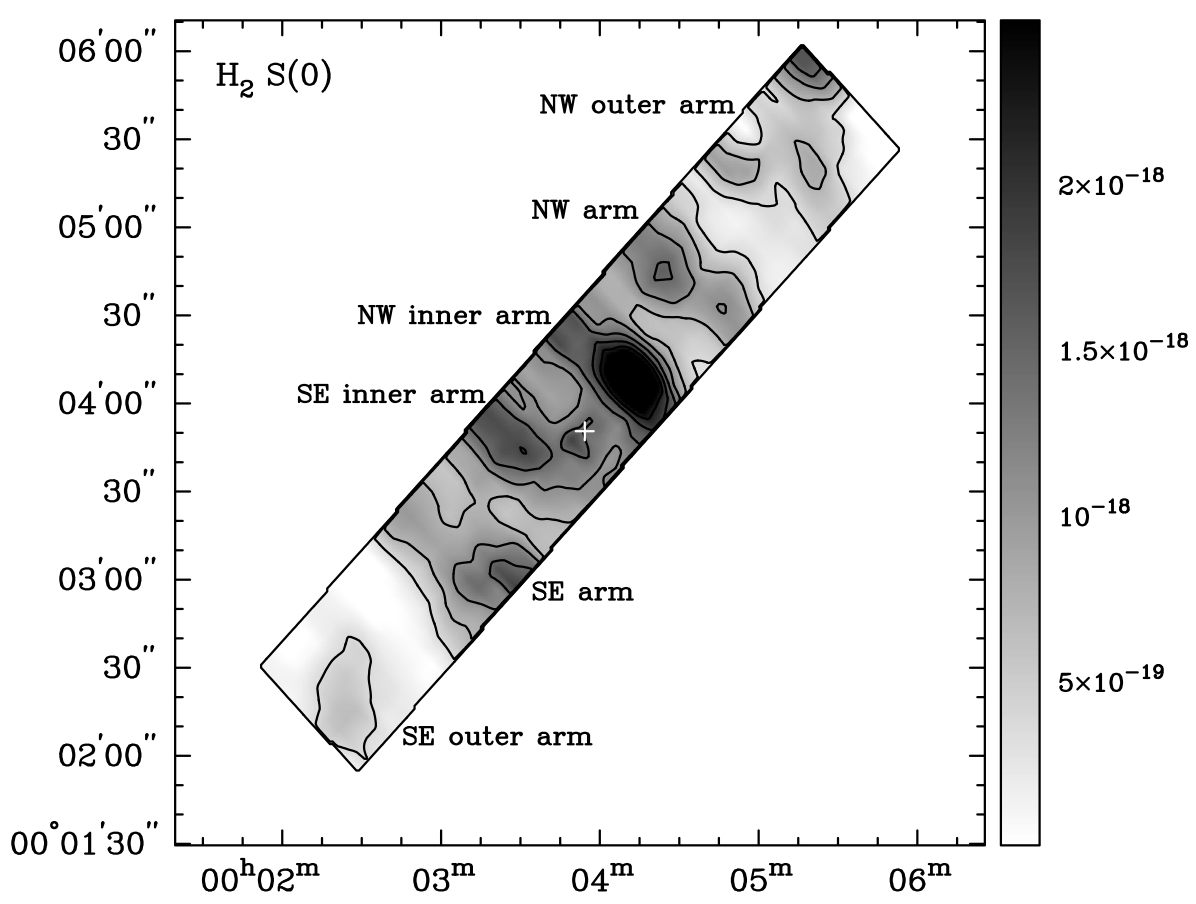
\includegraphics[width=8cm,angle=0]{bw_h2s0_contours.jpg}
\hspace{0.1in}
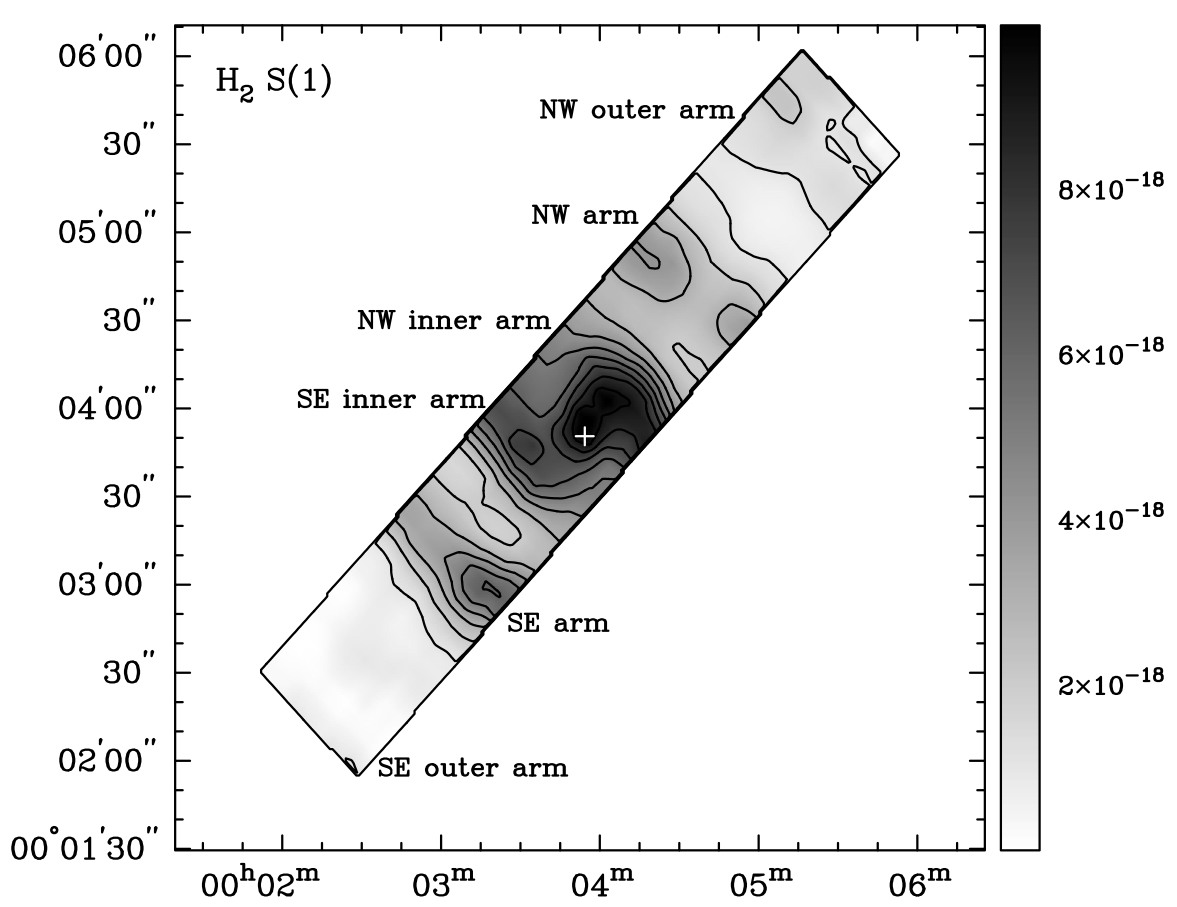
\includegraphics[width=8cm,angle=0]{bw_h2s1_contours.jpg}}}
\end{figure}
\begin{figure}[!h]
\centerline{\hbox{\hspace{0.0in}
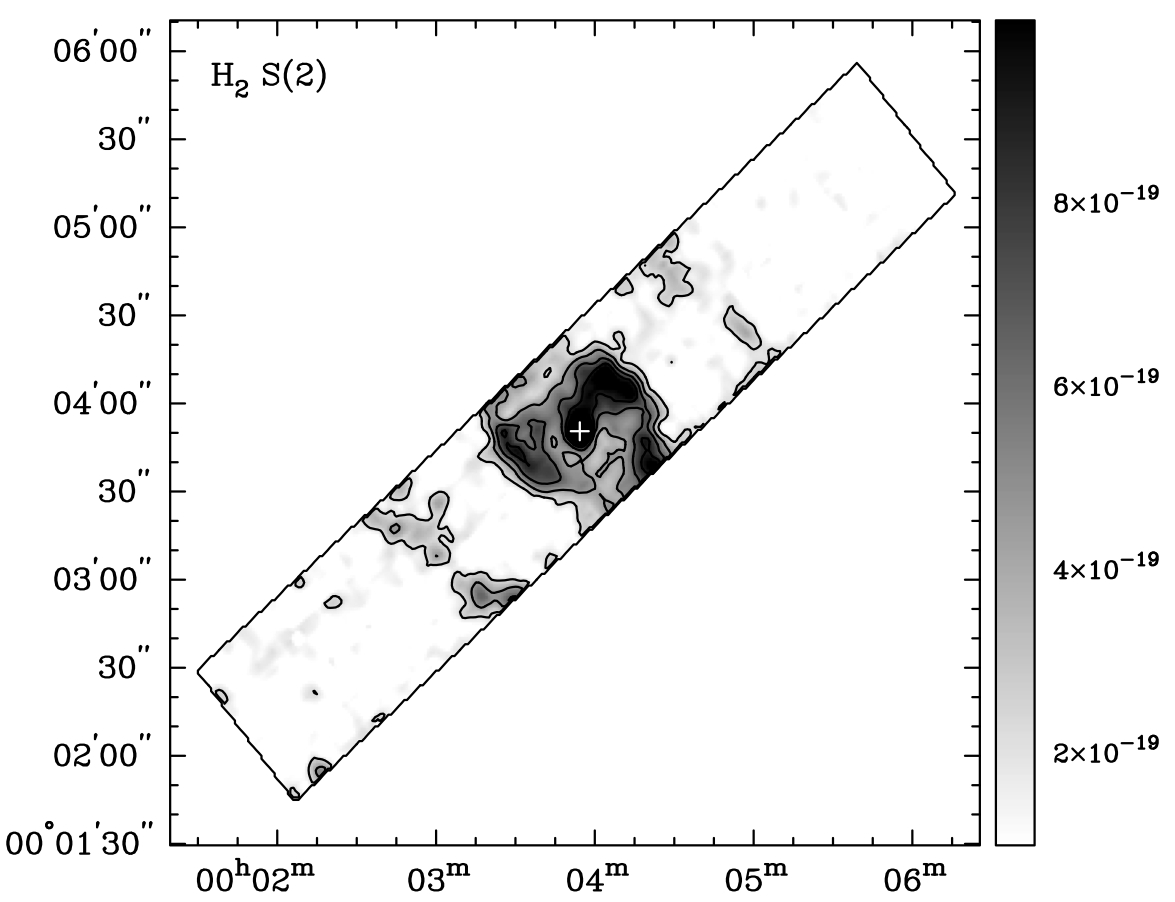
\includegraphics[width=8cm,angle=0]{bw_h2s2_contours.jpg}
\hspace{0.1in}
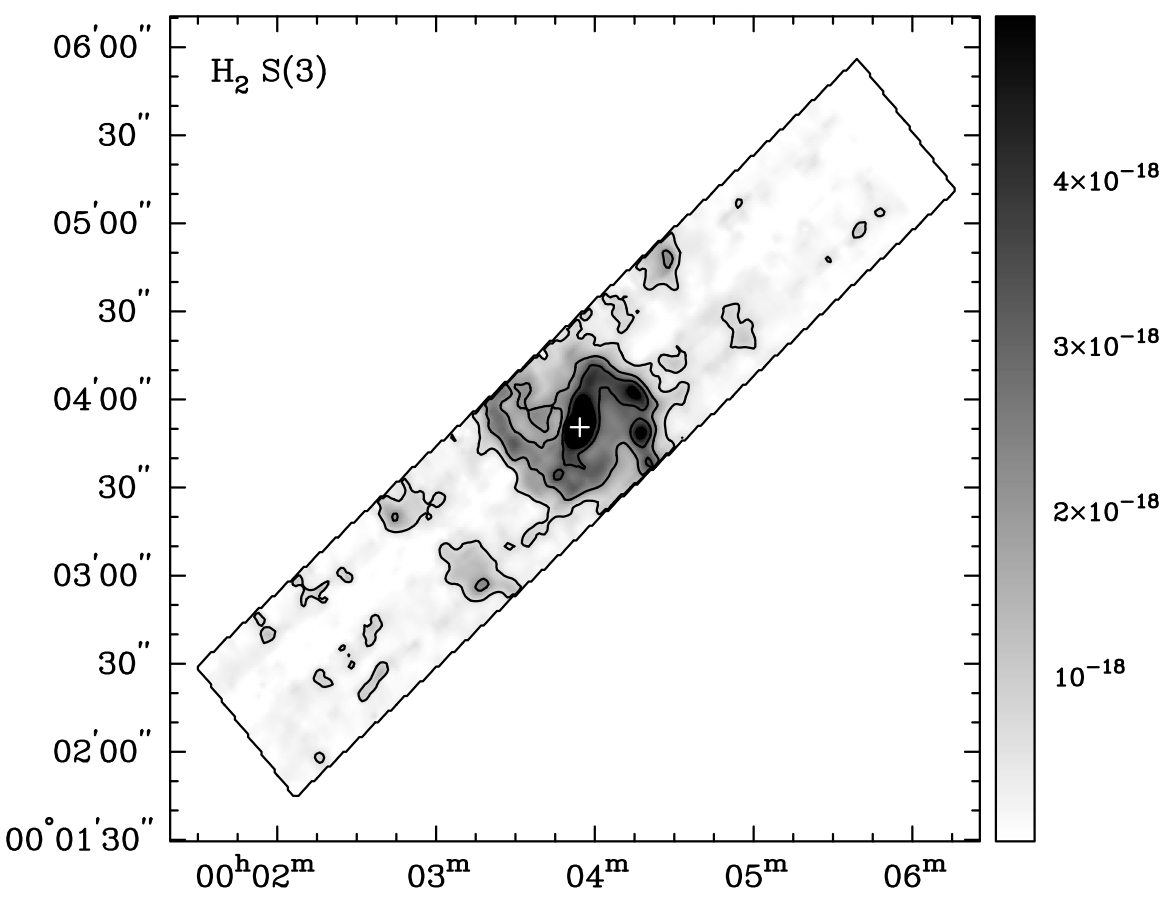
\includegraphics[width=8cm,angle=0]{bw_h2s3_contours.jpg}}}
\end{figure}
\begin{figure}[!h]
\centerline{\hbox{\hspace{0.0in}
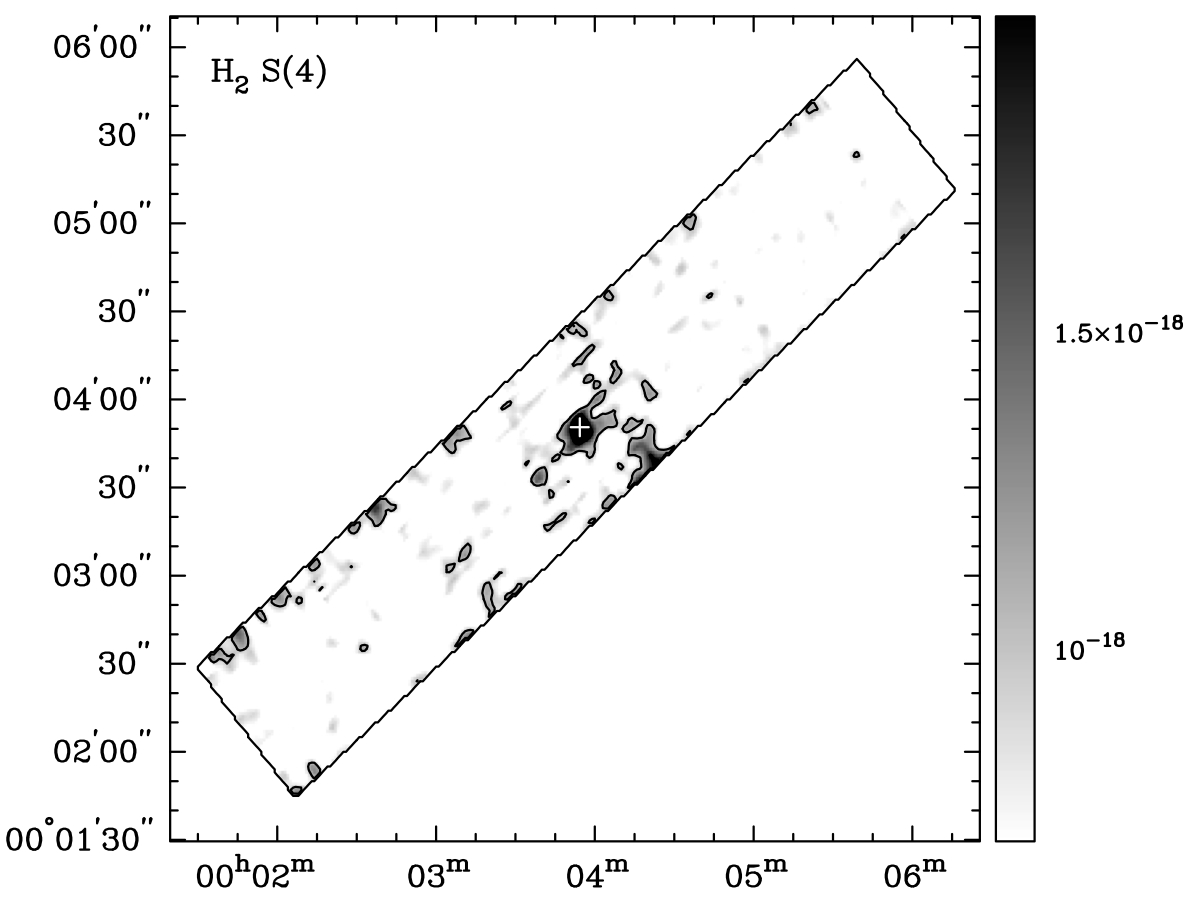
\includegraphics[width=8cm,angle=0]{bw_h2s4_contours.jpg}
\hspace{0.1in}
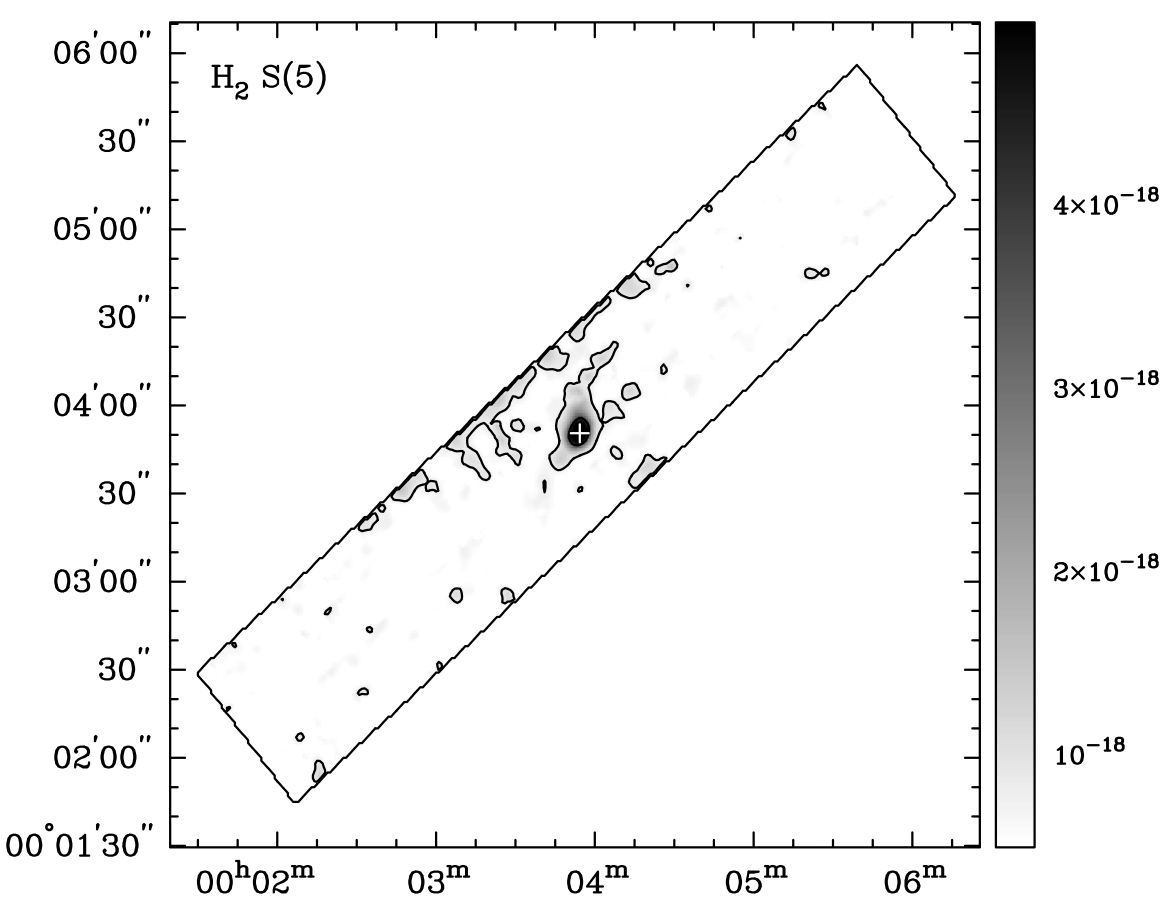
\includegraphics[width=8cm,angle=0]{bw_h2s5_contours.jpg}}}
\end{figure}
\begin{figure}
\caption{Maps of the $\mathrm{H_2}$ S(0) ($top$ $left$), $\mathrm{H_2}$ S(1) ($top$ $right$), $\mathrm{H_2}$ S(2) ($middle$ $left$), $\mathrm{H_2}$ S(3) ($middle$ $right$), $\mathrm{H_2}$ S(4) ($bottom$ $left$), and $\mathrm{H_2}$ S(5) ($bottom$ $right$) intensity across the SL and LL strips that we mapped with the Spitzer IRS.  The $\mathrm{H_2}$ S(0) and $\mathrm{H_2}$ S(1) maps are created from the LL data cubes. 
%The resolution of the $\mathrm{H_2}$ S(0) and $\mathrm{H_2}$ S(1) maps are 10$\farcs$2 and 6$\farcs$17, respectively.   
The $\mathrm{H_2}$ S(2), $\mathrm{H_2}$ S(3), $\mathrm{H_2}$ S(4), and $\mathrm{H_2}$ S(5) maps are created from the SL data cube.  
%The resolution of the $\mathrm{H_2}$ S(2), $\mathrm{H_2}$ S(3), $\mathrm{H_2}$ S(4), and $\mathrm{H_2}$ S(5) maps are 4$\farcs$37, 3$\farcs$44, 2$\farcs$85, and 2$\farcs$46, respectively.  
The grey-scale is in units of W/$\mathrm{m^2}$.  Contour levels are at 2.9 $\times$ ${10^{-18}}$, 2.2 $\times$ ${10^{-18}}$, 1.8 $\times$ ${10^{-18}}$, 1.5 $\times$ ${10^{-18}}$, 1.1 $\times$ ${10^{-18}}$, 7.3 $\times$ ${10^{-19}}$, and 3.7 $\times$ ${10^{-19}}$ W/$\mathrm{m^2}$ for $\mathrm{H_2}$ S(0); 9.6 $\times$ ${10^{-18}}$, 8.6 $\times$ ${10^{-18}}$, 7.5 $\times$ ${10^{-18}}$, 6.4 $\times$ ${10^{-18}}$, 5.4 $\times$ ${10^{-18}}$, 4.3 $\times$ ${10^{-18}}$, 3.2 $\times$ ${10^{-18}}$, 2.1 $\times$ ${10^{-18}}$and 1.1 $\times$ ${10^{-18}}$ W/$\mathrm{m^2}$ for $\mathrm{H_2}$ S(1); 1.1 $\times$ ${10^{-18}}$, 8.9 $\times$ ${10^{-19}}$, 6.7 $\times$ ${10^{-19}}$, 4.4 $\times$ ${10^{-19}}$, and 2.2 $\times$ ${10^{-19}}$ W/$\mathrm{m^2}$ for $\mathrm{H_2}$ S(2); 1.21 $\times$ ${10^{-17}}$, 9.4 $\times$ ${10^{-18}}$, 6.7 $\times$ ${10^{-18}}$, 4.0 $\times$ ${10^{-18}}$, and 1.3 $\times$ ${10^{-18}}$ W/$\mathrm{m^2}$ for $\mathrm{H_2}$ S(3);  2.0 $\times$ ${10^{-18}}$and 1.0 $\times$ ${10^{-18}}$ W/$\mathrm{m^2}$ for $\mathrm{H_2}$ S(4); 7.3 $\times$ ${10^{-18}}$, 4.0 $\times$ ${10^{-18}}$, and 8.0 $\times$ ${10^{-19}}$ W/$\mathrm{m^2}$ for $\mathrm{H_2}$ S(5).  The vertical axis is the right ascension and the horizontal axis is the declination.  Note that in all of the maps, north is up and west is to the left.  The box around the intensity maps represents the SL or LL strip that we mapped.\label{fig1}}

%Contours are spaced at 10\%  of the peak flux (6.074 x 10^{-9} W/${m^2}$/sr for $\mathrm{H_2}$S(0) and 1.701 x 10^{-8} W/${m^2}$/sr for $\mathrm{H_2}$S(1)) in each image.  The box around the contour represents the radial strip that was mapped in the IRS LL module.  Note that in all of the maps, north is up and west is to the left.\label{fig1}}

\end{figure}
\clearpage


%\begin{figure}[!h]
%\centerline{\hbox{\hspace{0.0in}
%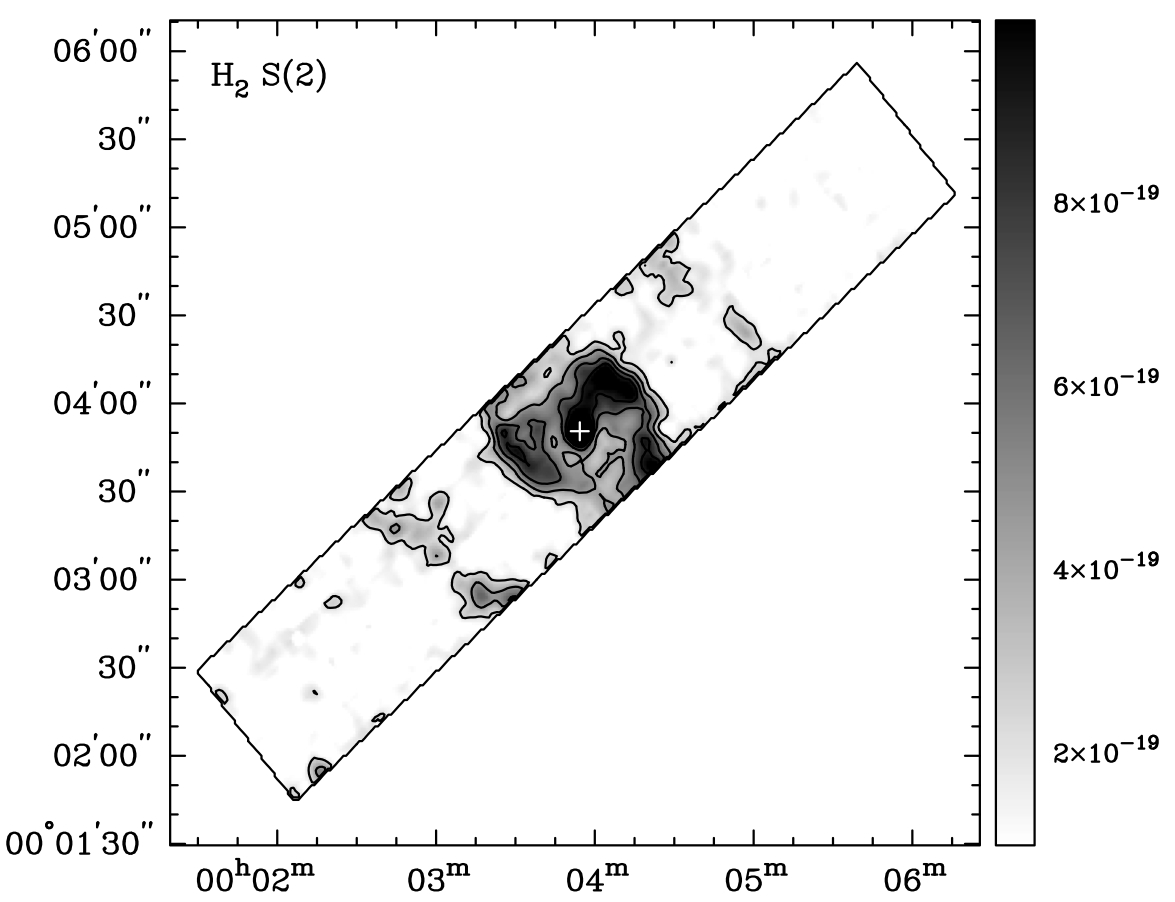
\includegraphics[width=8cm,angle=0]{bw_h2s2_contours.jpg}
%\hspace{0.1in}
%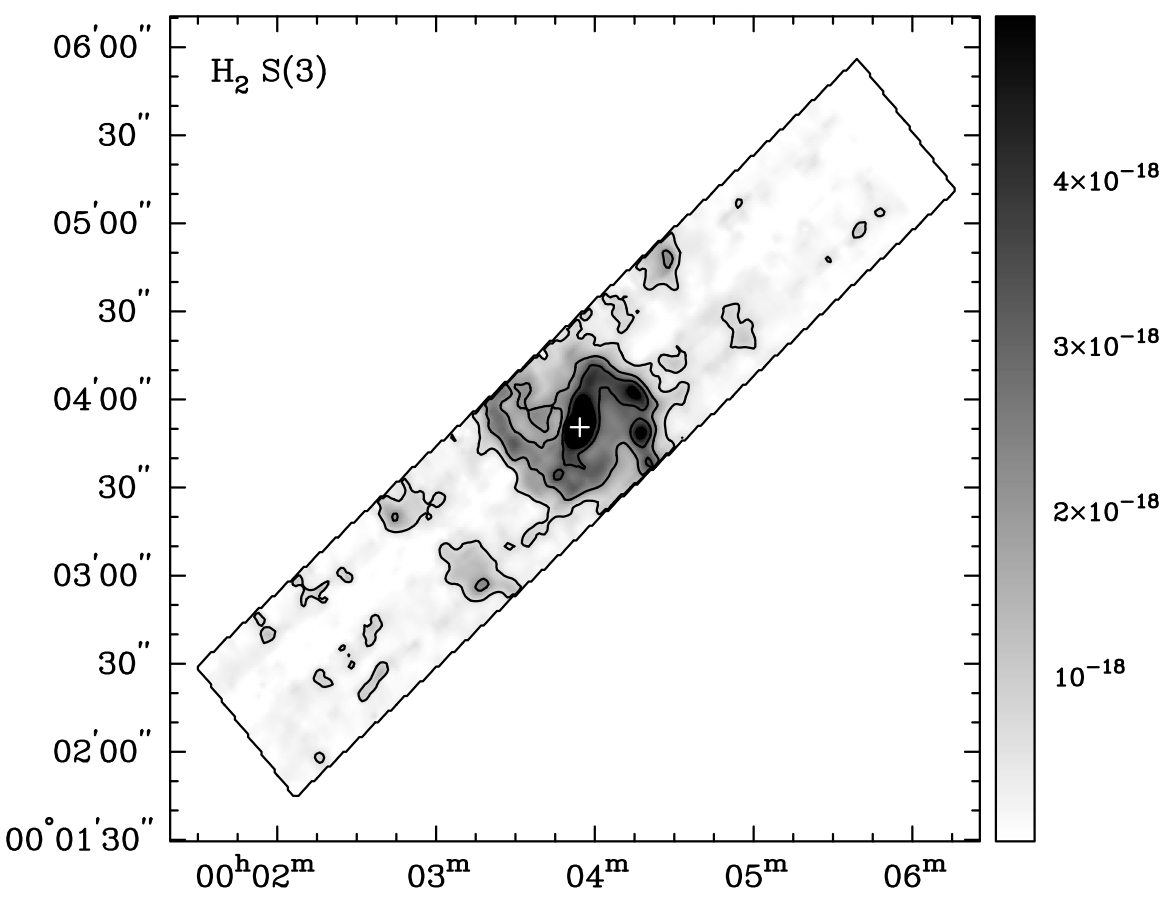
\includegraphics[width=8cm,angle=0]{bw_h2s3_contours.jpg}}}
%\end{figure}

%\begin{figure}[!h]
%\centerline{\hbox{\hspace{0.0in}
%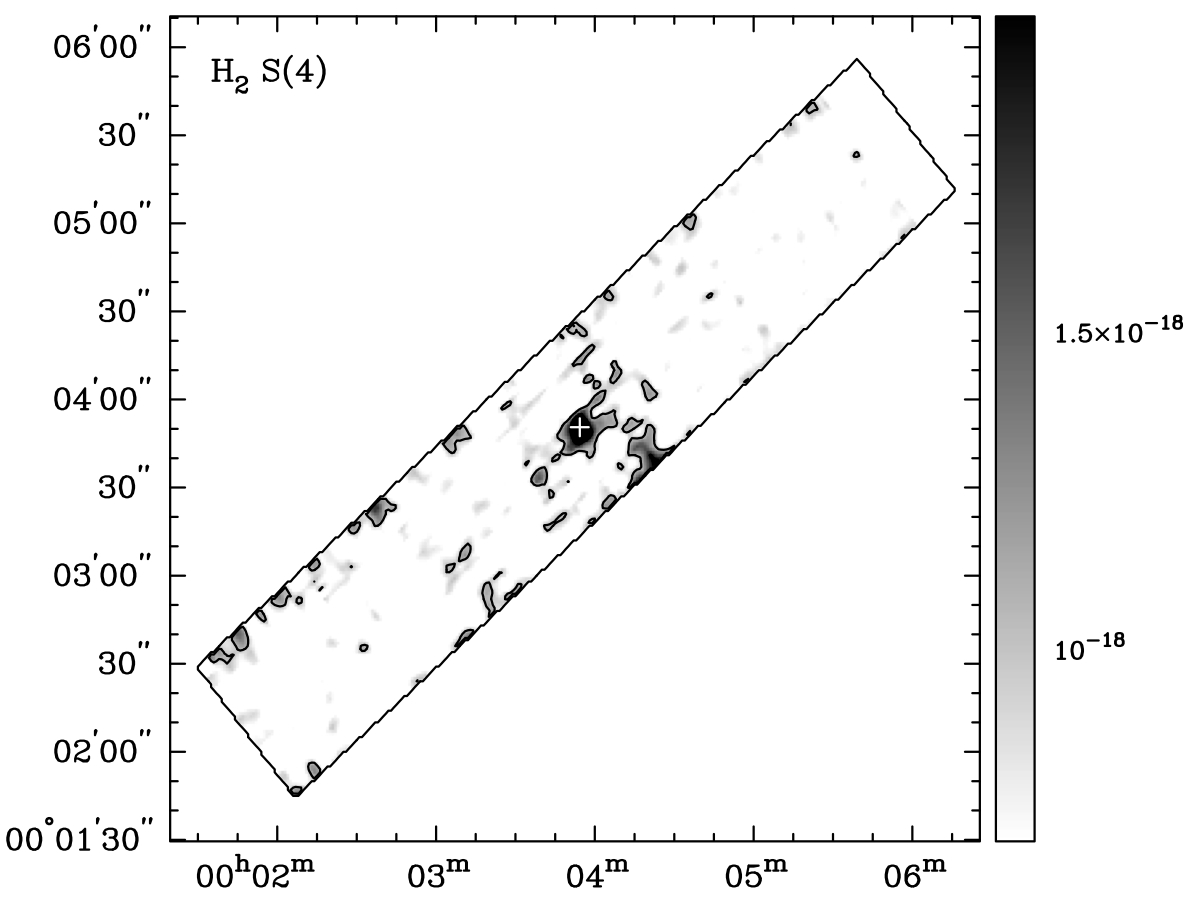
\includegraphics[width=8cm,angle=0]{bw_h2s4_contours.jpg}
%\hspace{0.1in}
%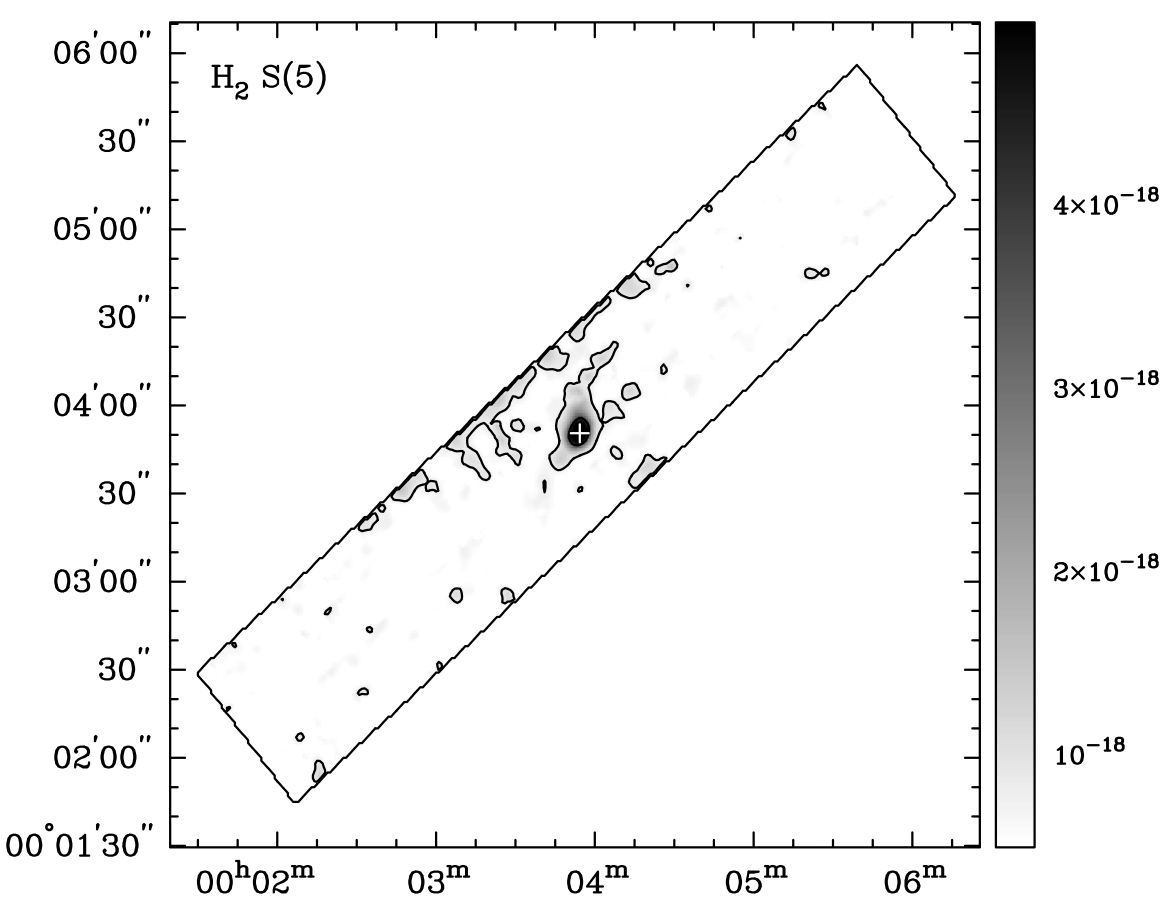
\includegraphics[width=8cm,angle=0]{bw_h2s5_contours.jpg}}}
%\caption{Maps of $\mathrm{H_2}$ S(2) (top left), $\mathrm{H_2}$ S(3) (top right), $\mathrm{H_2}$ S(4) (bottom left), and $\mathrm{H_2}$ S(5) (bottom right) emission intensity.  All four maps are created from the SL data cube.  The resolution of the $\mathrm{H_2}$ S(2), $\mathrm{H_2}$ S(3), $\mathrm{H_2}$ S(4), and $\mathrm{H_2}$ S(5) maps are 4".37, 3".44, 2".85, and 2".46, respectively.  The grey-scale is in units of W/$\mathrm{m^2}$.  Contours levels are at 1.1 x ${10^{-18}}$, 8.9 x ${10^{-19}}$, 6.7 x ${10^{-19}}$, 4.4 x ${10^{-19}}$, and 2.2 x ${10^{-19}}$ W/$\mathrm{m^2}$ for $\mathrm{H_2}$ S(2); 1.21 x ${10^{-17}}$, 9.4 x ${10^{-18}}$, 6.7 x ${10^{-18}}$, 4.0 x ${10^{-18}}$, and 1.3 x ${10^{-18}}$ W/$\mathrm{m^2}$ for $\mathrm{H_2}$ S(3);  2.0 x ${10^{-18}}$and 1.0 x ${10^{-18}}$ W/$\mathrm{m^2}$ for $\mathrm{H_2}$ S(4); 7.3 x ${10^{-18}}$, 4.0 x ${10^{-18}}$, and 8.0 x ${10^{-19}}$ W/$\mathrm{m^2}$ for $\mathrm{H_2}$ S(5).  The vertical axis is the right ascension and the horizontal axis is the declination.  The box around the intensity maps represents the SL strip that was mapped.\label{fig2}}
%\end{figure}

\clearpage

\begin{figure}[!h]
\centerline{\hbox{ \hspace{0.0in} 
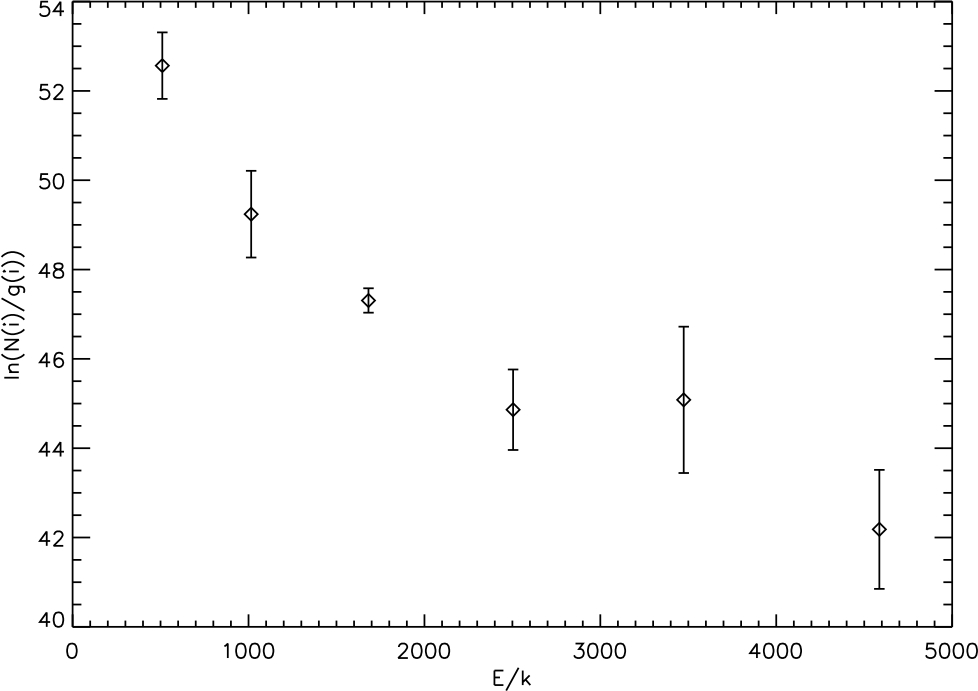
\includegraphics[width=8cm,angle=0]{region1.jpg}
\hspace{0.1in}
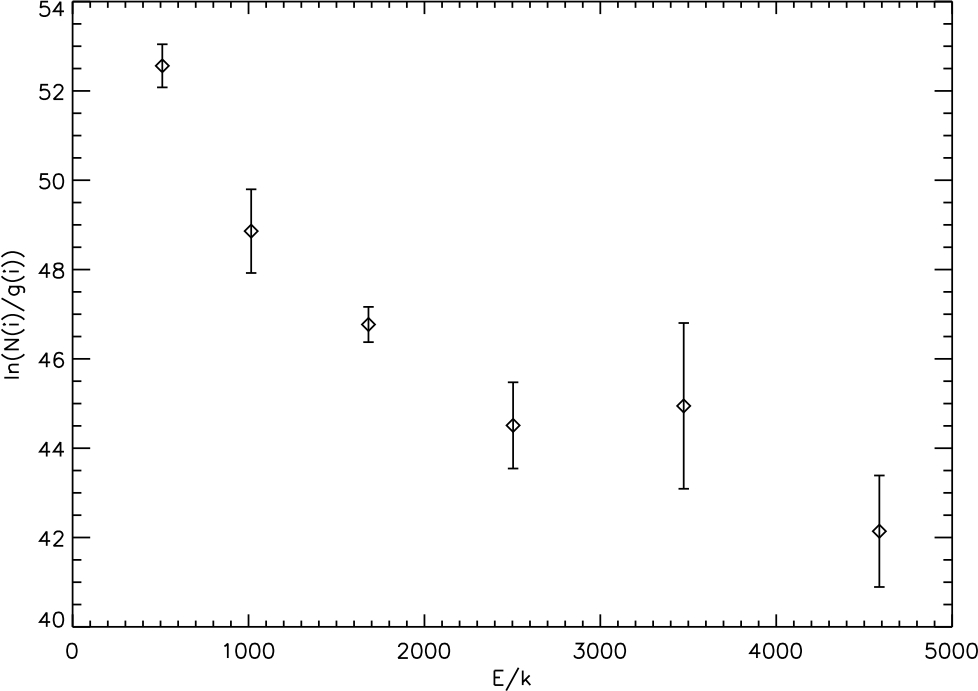
\includegraphics[width=8cm,angle=0]{region3.jpg}}}
\end{figure}

\begin{figure}[!h]
\centerline{\hbox{\hspace{0.0in}
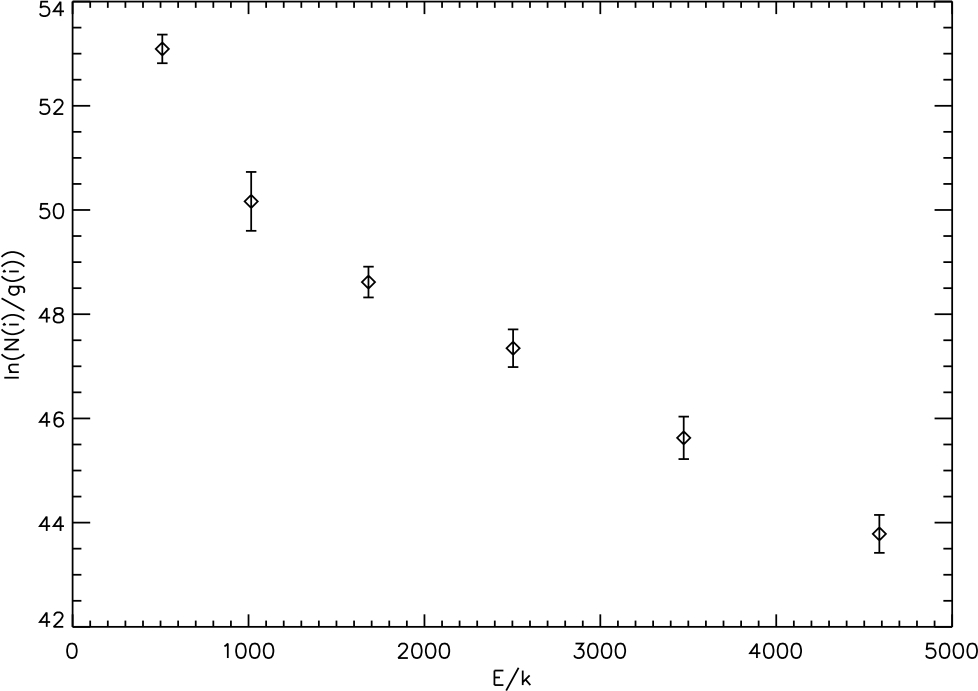
\includegraphics[width=8cm,angle=0]{region2.jpg}}}
\caption{Excitation diagrams taken from 3 different regions along the M51 strip.  The top two excitation diagrams are taken from regions within the southeast and northwest spiral arms that are 10$\farcs$2 in diameter (1.13 $\times$ $\mathrm{10^5}$ $\mathrm{pc^2}$) and centered at (RA, Dec) of (202.45, 47.21) and (202.49, 47.18), respectively. The excitation diagram at the bottom is taken from from the nuclear region.  The aperture is 10$\farcs$2 in diameter (1.13 $\times$ $\mathrm{10^5}$ $\mathrm{pc^2}$), centered at (RA, Dec) of (202.47, 47.19).
\label{fig2}}
\end{figure}




\clearpage

\begin{figure}[!h]
\centerline{\hbox{\hspace{0.0in}
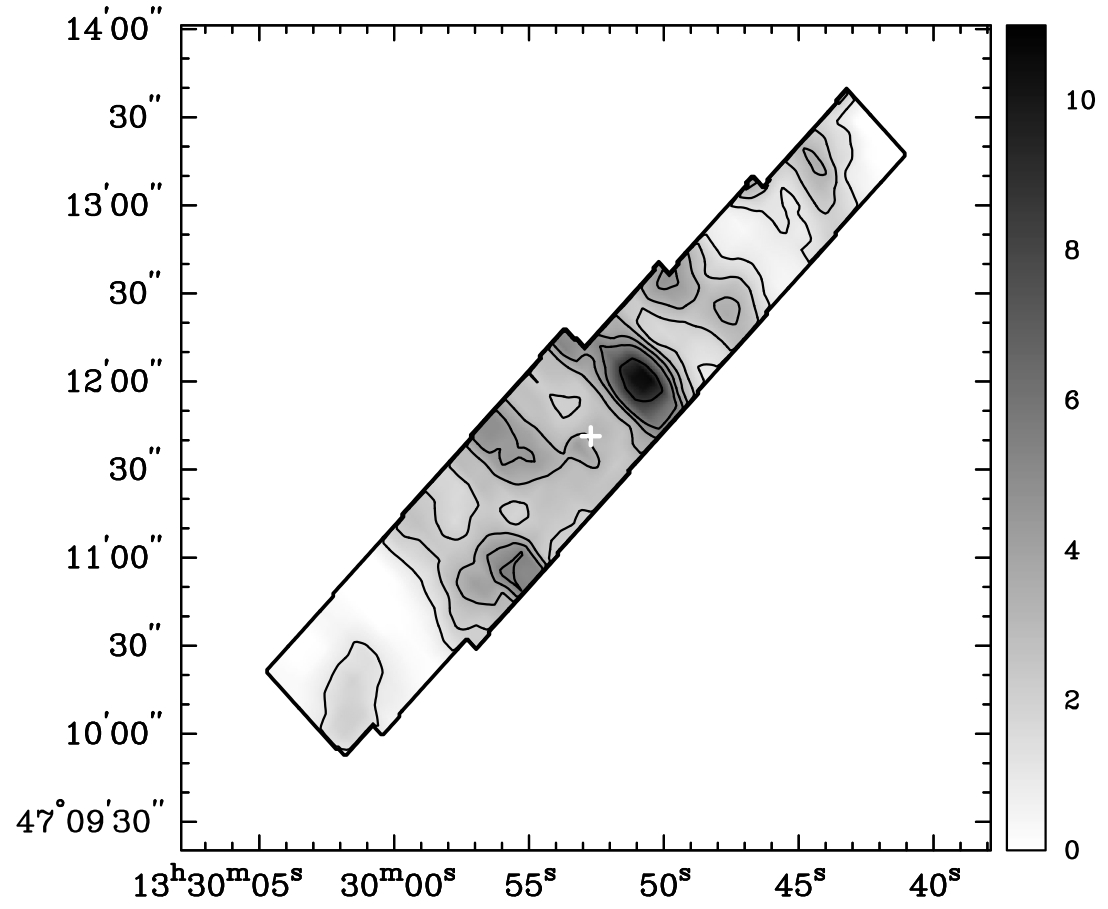
\includegraphics[width=8cm,angle=0]{bw_warm_h2_mass.jpg}
\hspace{0.1in}
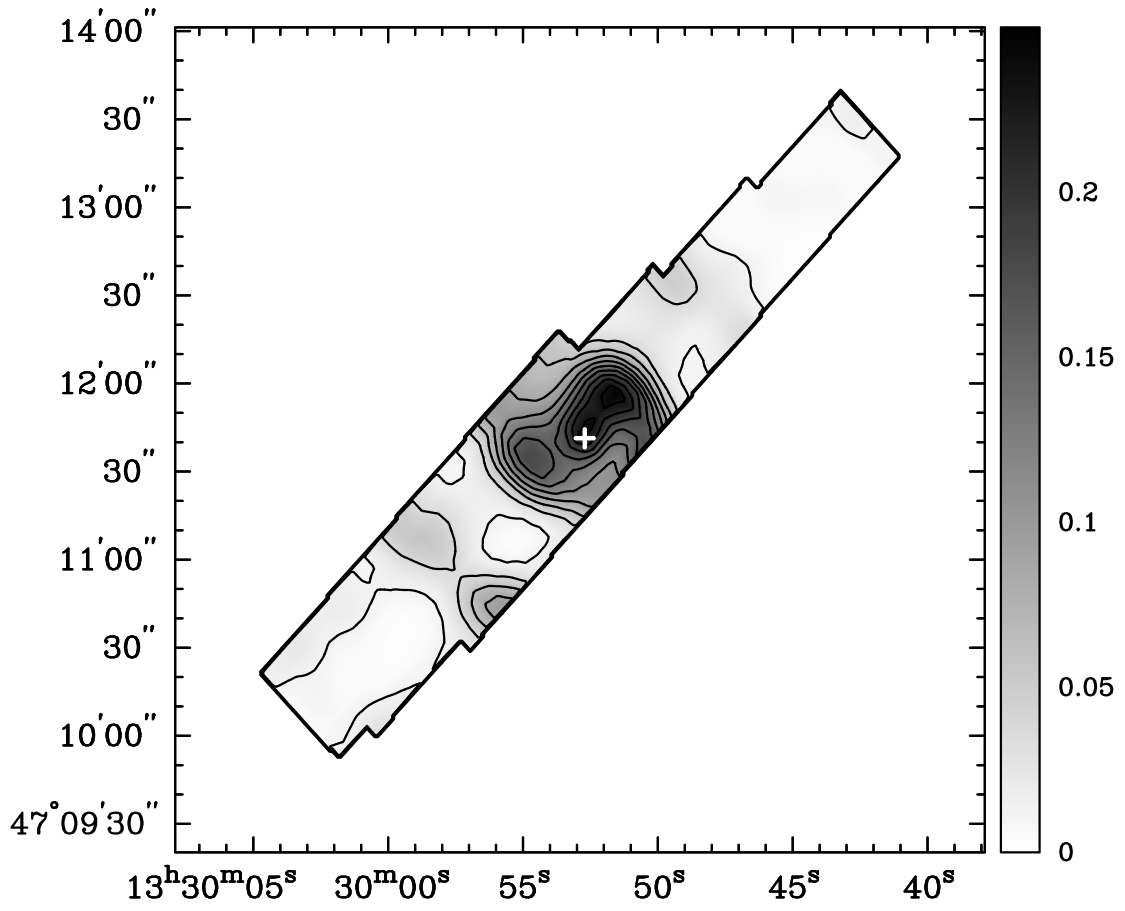
\includegraphics[width=8cm,angle=0]{bw_hot_h2_mass.jpg}}}
\caption{Shown are the warm (T = 100 $-$ 300 K) $\mathrm{H_2}$ ($left$) and hot (T = 400 $-$ 1000 K) $\mathrm{H_2}$ ($right$) mass distributions.  The mass distributions are in units of $\mathrm{M_\sun}$/$\mathrm{pc^2}$.   Contours are overplotted for clarity.  The warm $\mathrm{H_2}$ mass contour levels are at 8.85, 5.55, 4.43, 3.32, 2.21, and 1.10 $\mathrm{M_\sun}$/$\mathrm{pc^2}$.  The hot $\mathrm{H_2}$ contour levels are at 10 \% of 0.25 $\mathrm{M_\sun}$/$\mathrm{pc^2}$.  The hot $\mathrm{H_2}$ mass distribution is derived from the fit to the $\mathrm{H_2}$ S(2) $-$ $\mathrm{H_2}$ S(5) lines and the warm $\mathrm{H_2}$ mass distribution is derived from the fit to the $\mathrm{H_2}$ S(0) $-$ $\mathrm{H_2}$ S(2) lines, corrected for the contribution of the hot $\mathrm{H_2}$ mass phase.  \label{fig3}}
\end{figure}

\clearpage

\begin{figure}[!h]
\centerline{\hbox{\hspace{0.0in}
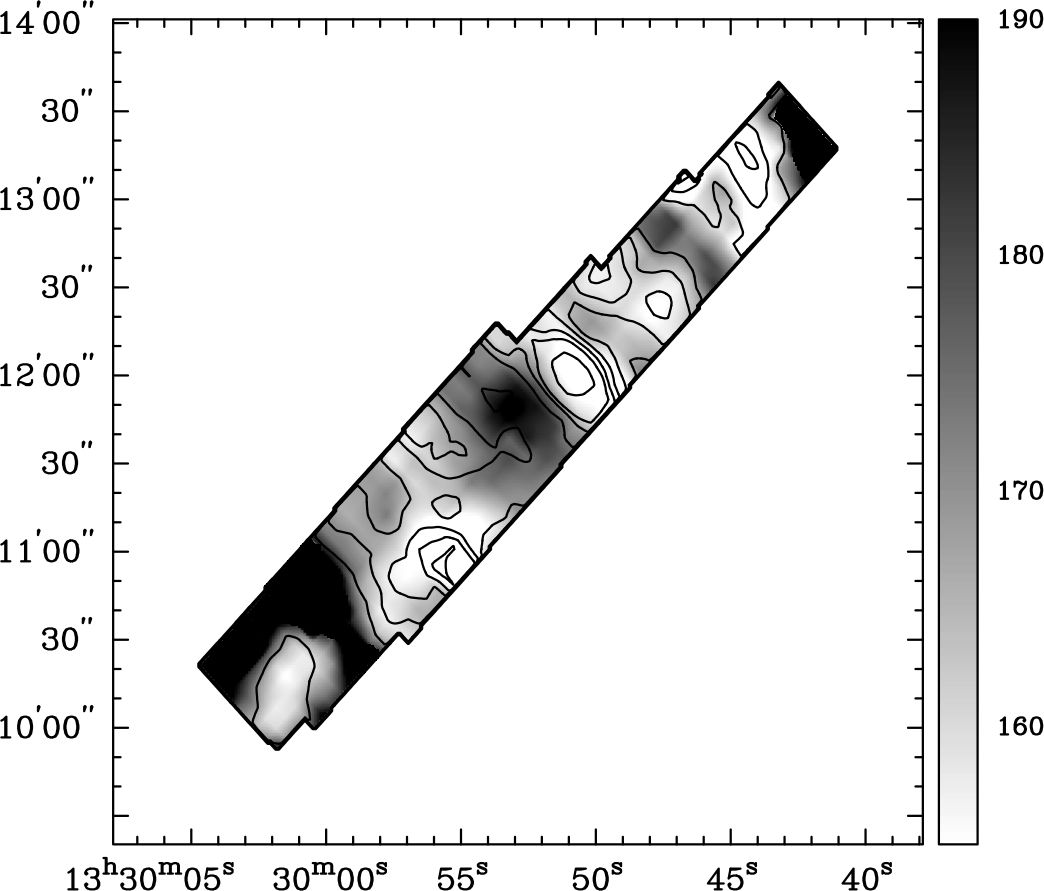
\includegraphics[width=8cm,angle=0]{bw_warm_h2_fill.jpg}}}
\caption{The warm (T = 100 $-$ 300 K) $\mathrm{H_2}$ mass distribution compared to the warm $\mathrm{H_2}$ excitation-temperature.  The warm $\mathrm{H_2}$ excitation-temperature and mass distributions are derived from the fit to the excitation diagrams across the strip for the $\mathrm{H_2}$ S(0) $-$ $\mathrm{H_2}$ S(2) lines, corrected for the contribution of the hot (T = 400 $-$ 1000 K) $\mathrm{H_2}$ phase.  Mass density contour levels are at 8.85, 5.55, 4.43, 3.32, 2.21, and 1.10 $\mathrm{M_\sun}$/$\mathrm{pc^2}$ (same as in Figure 3).
% Contours represent the mass within a 3.61 $\times$ ${10^{4}}$ $\mathrm{pc^2}$ area. 
The grey-scale represents the excitation-temperature distribution (in units of Kelvin).  The non-rectangular shape to the map is due to the slight offset of the $Spitzer$ IRS SL strip relative to the LL strip.  \label{fig4}}
\end{figure}

\clearpage
\begin{figure}[!h]
\centerline{\hbox{\hspace{0.0in}
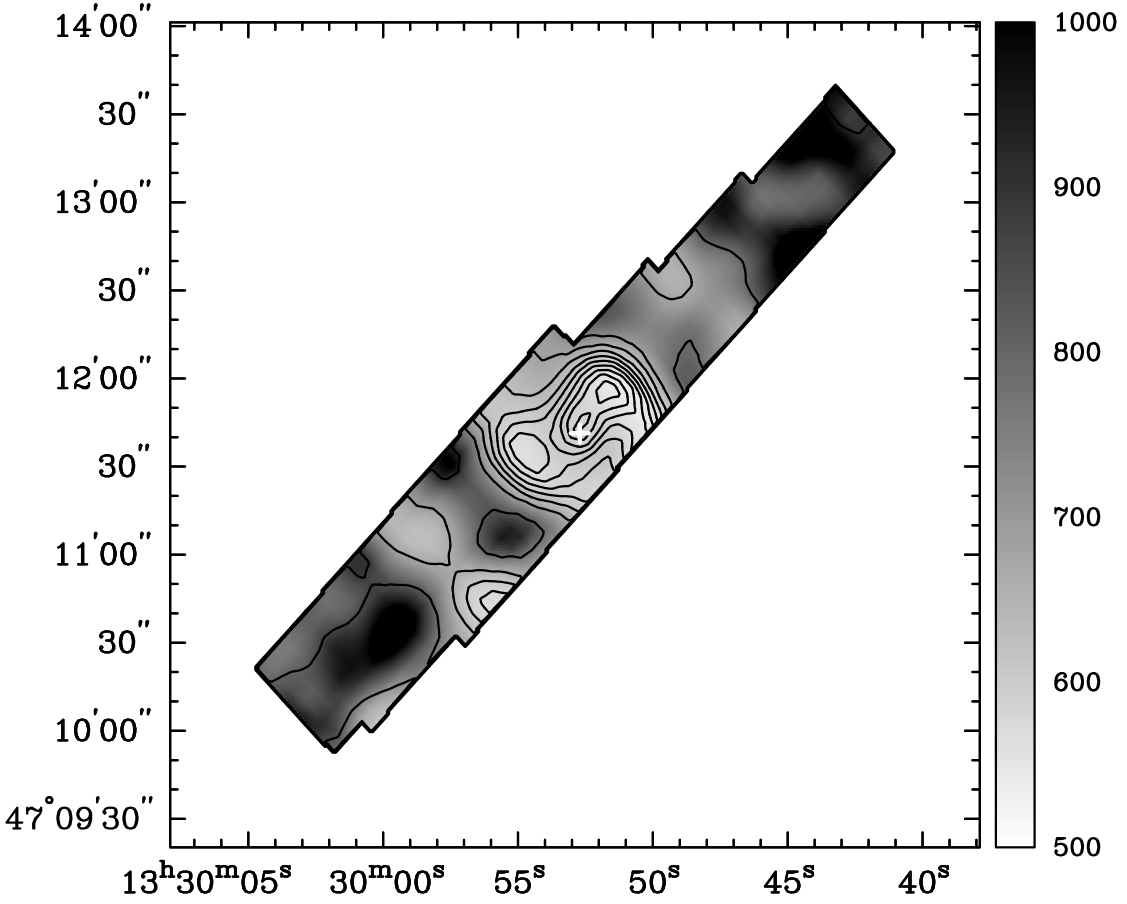
\includegraphics[width=8cm,angle=0]{bw_hot_h2.jpg}}}
\caption{The hot (T = 400 $-$ 1000 K) $\mathrm{H_2}$ mass distribution compared to the hot $\mathrm{H_2}$ excitation-temperature.  The hot $\mathrm{H_2}$ excitation-temperature and mass distributions are derived from the fit to the excitation diagrams across the strip for the $\mathrm{H_2}$ S(2) $-$ $\mathrm{H_2}$ S(5) lines.  Mass density contour levels are at 10\% of 0.25 $\mathrm{M_\sun}$/$\mathrm{pc^2}$ (same as in Figure 3). 
%Contours represent the amount of mass of the hot $\mathrm{H_2}$ within a 3.61 x 10^{4} $\mathrm{pc^2}$ area.  
The grey-scale represents the excitation-temperature distribution (in units of Kelvin).  Note that the due to lack of $\mathrm{H_2}$ detection from the higher $J$ lines at greater distances from the nucleus of NGC 5194, we are unable to map the hot $\mathrm{H_2}$ distributions across the entire strip as we have done for the warm $\mathrm{H_2}$ distribution.\label{fig5}}
\end{figure}

\clearpage
\begin{figure}[!h]
\centerline{\hbox{\hspace{0.0in}
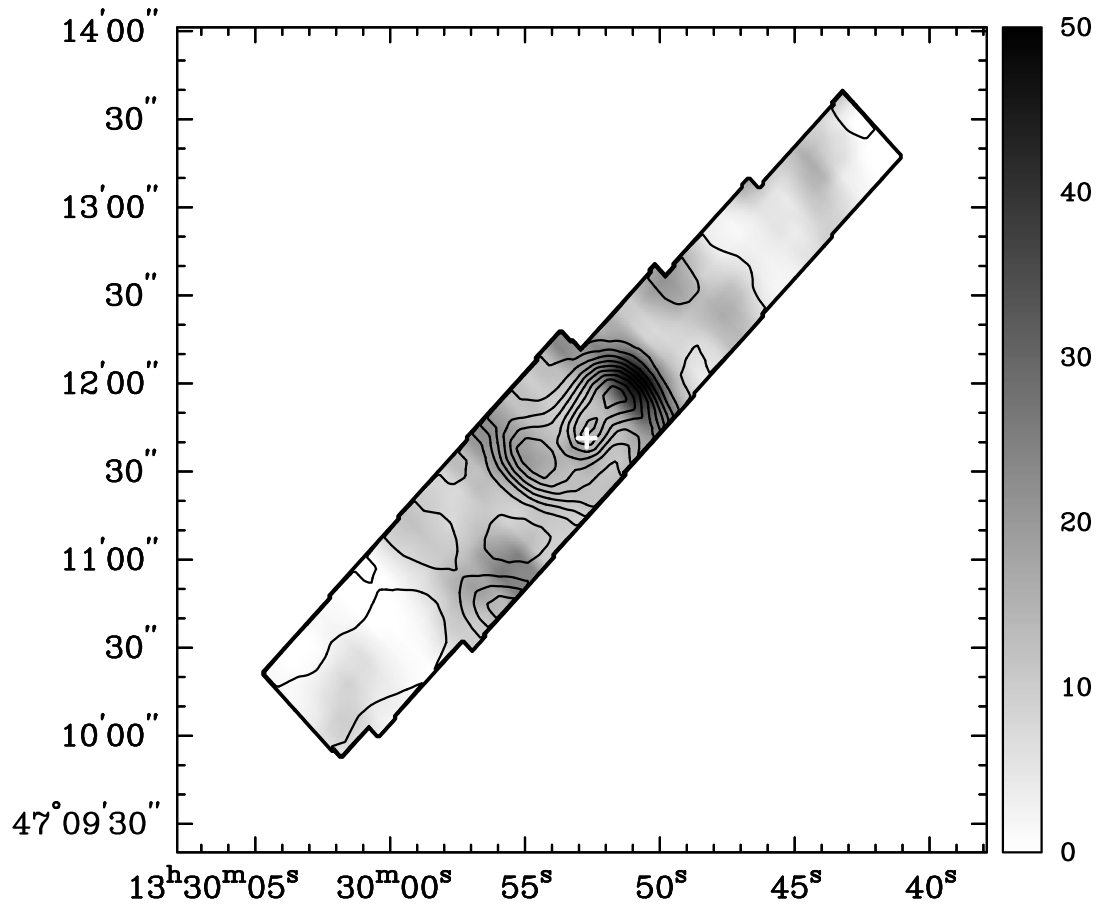
\includegraphics[width=8cm,angle=0]{bw_warm_v_hot.jpg}}}
\caption{The warm (T = 100 $-$ 300 K) $\mathrm{H_2}$ mass (in grey-scale) compared to the hot (T = 400 $-$ 1000 K) $\mathrm{H_2}$ mass (in contours).  Contours levels for the hot $\mathrm{H_2}$ mass distribution are at 10\% of the maximum mass density 0.25 $\mathrm{M_\sun}$/$\mathrm{pc^2}$. 
%Contours represent the amount of mass of the hot $\mathrm{H_2}$ within a 3.61 x ${10^{4}}$ $\mathrm{pc^2}$ area.  
The grey-scale is in units of $\mathrm{M_\sun}$/$\mathrm{pc^2}$.
% and also represents the amount of mass of the warm $\mathrm{H_2}$ within a 3.61 x ${10^{4}}$ $\mathrm{pc^2}$ area. 
\label{fig6}}
\end{figure}


\clearpage


\begin{figure}[!h]
\centerline{\hbox{\hspace{0.0in}
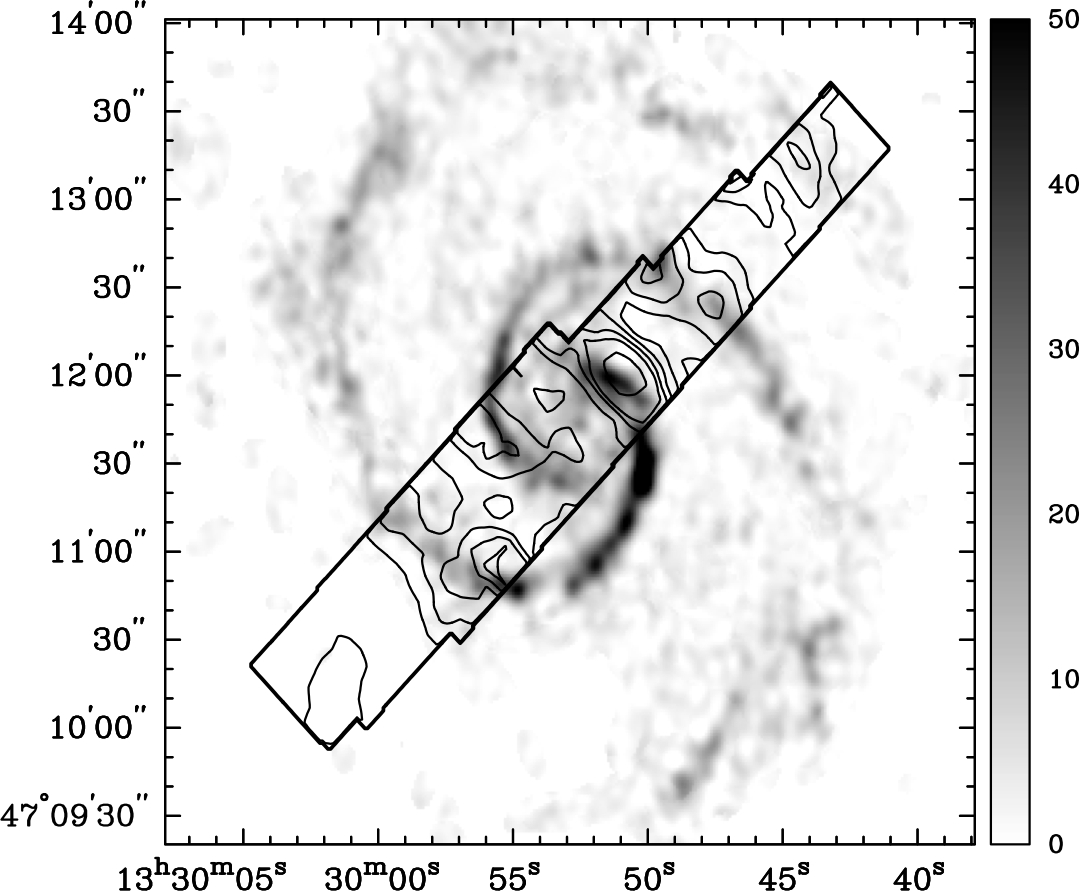
\includegraphics[width=8cm,angle=0]{bw_co_v_warm.jpg}
\hspace{0.1in}
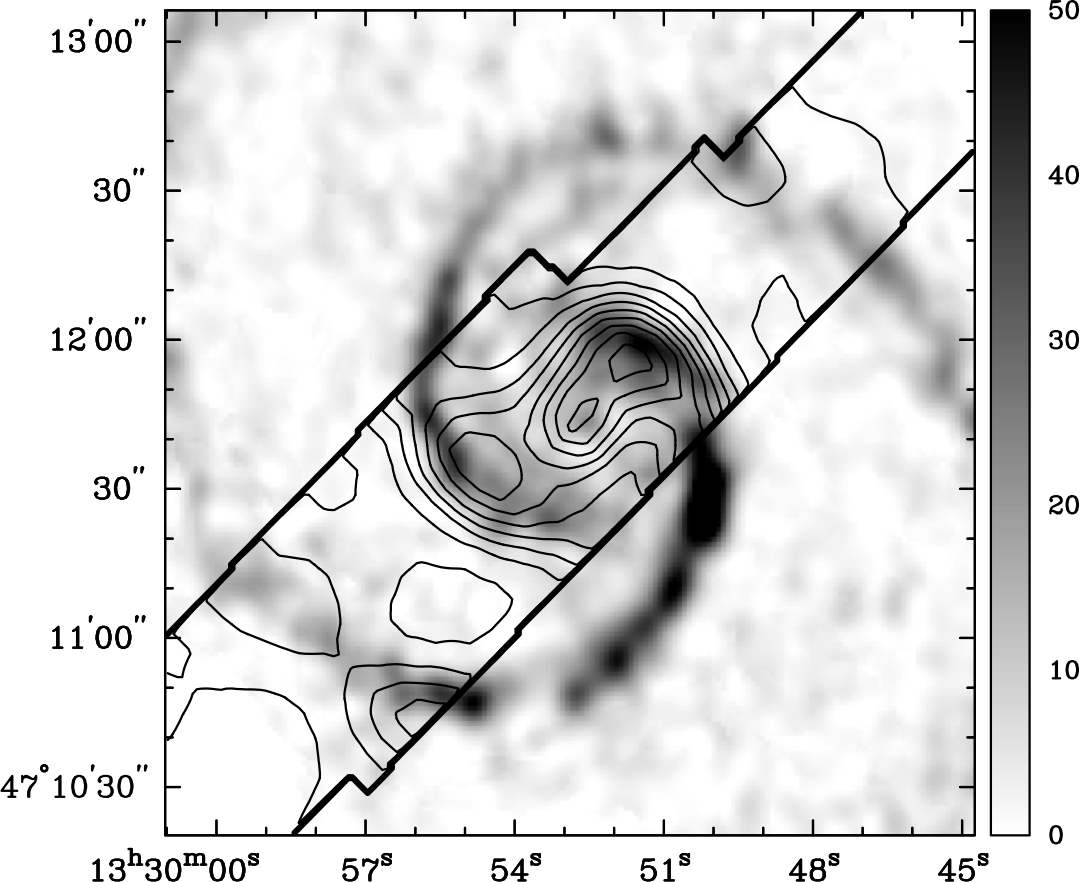
\includegraphics[width=8cm,angle=0]{bw_co_v_hot.jpg}}}
\caption{$Left$: Comparison of  CO intensity (in grey-scale) to the warm (T = 100 $-$ 300 K) $\mathrm{H_2}$ mass (in contours).  The CO intensity is in units of Jy beam $\mathrm{s^{-1}}$. The warm $\mathrm{H_2}$ mass contours are the same as in Figures 3 and 4.  $Right$: Comparison of CO intensity (in grey-scale) to the hot (T = 400 $-$ 1000 K) $\mathrm{H_2}$ mass (in contours).  The CO intensity is in units of Jy beam $\mathrm{s^{-1}}$. The hot $\mathrm{H_2}$ mass contours are the same as in Figures 3 and 5.
\label{fig7}}
\end{figure}

\clearpage


\begin{figure}[!h]
\centerline{\hbox{ \hspace{0.0in} 
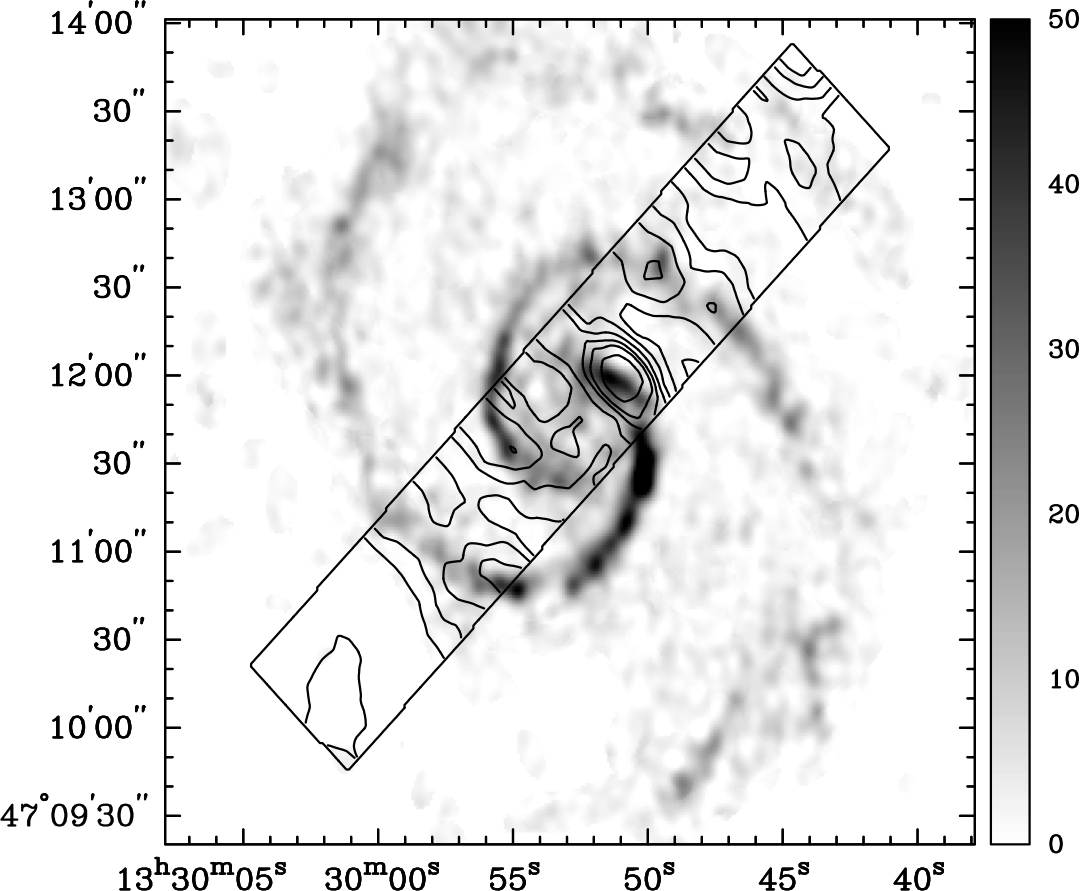
\includegraphics[width=8cm,angle=0]{bw_co_h2s0.jpg}
\hspace{0.1in}
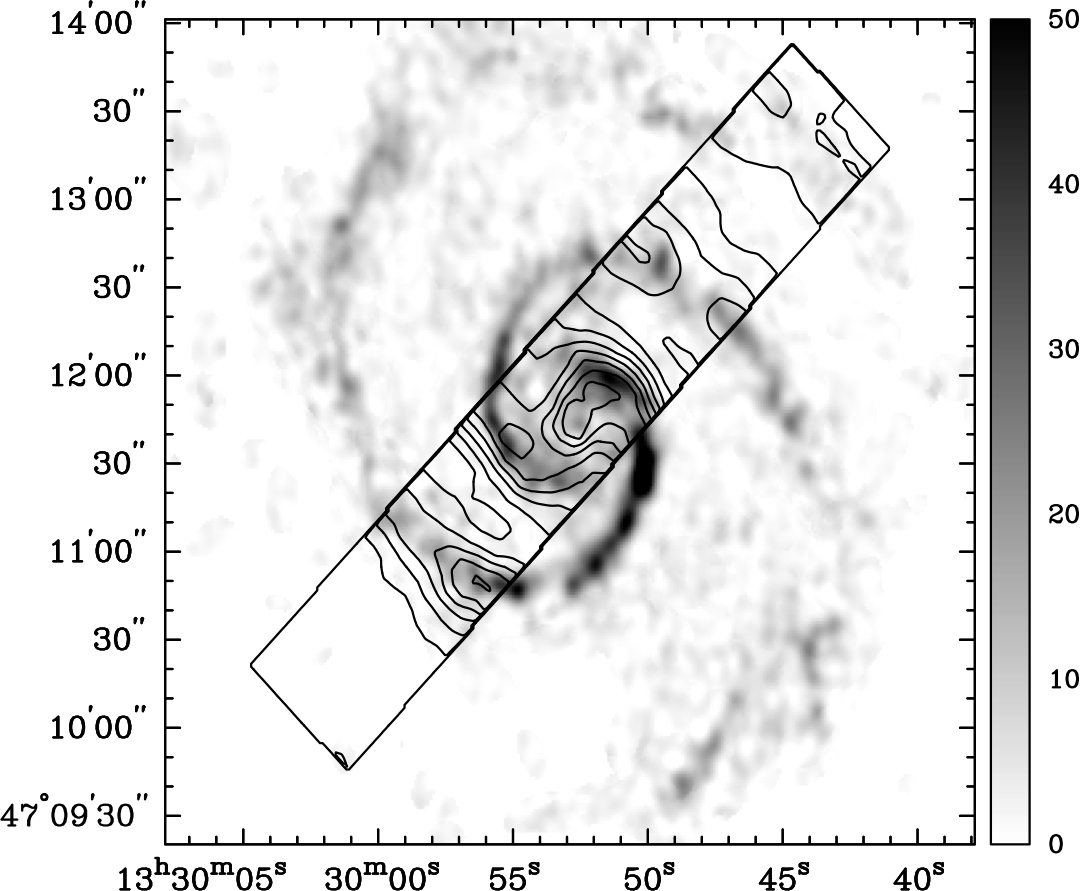
\includegraphics[width=8cm,angle=0]{bw_co_h2s1.jpg}}}
\end{figure}

\begin{figure}[!h]
\centerline{\hbox{\hspace{0.0in}
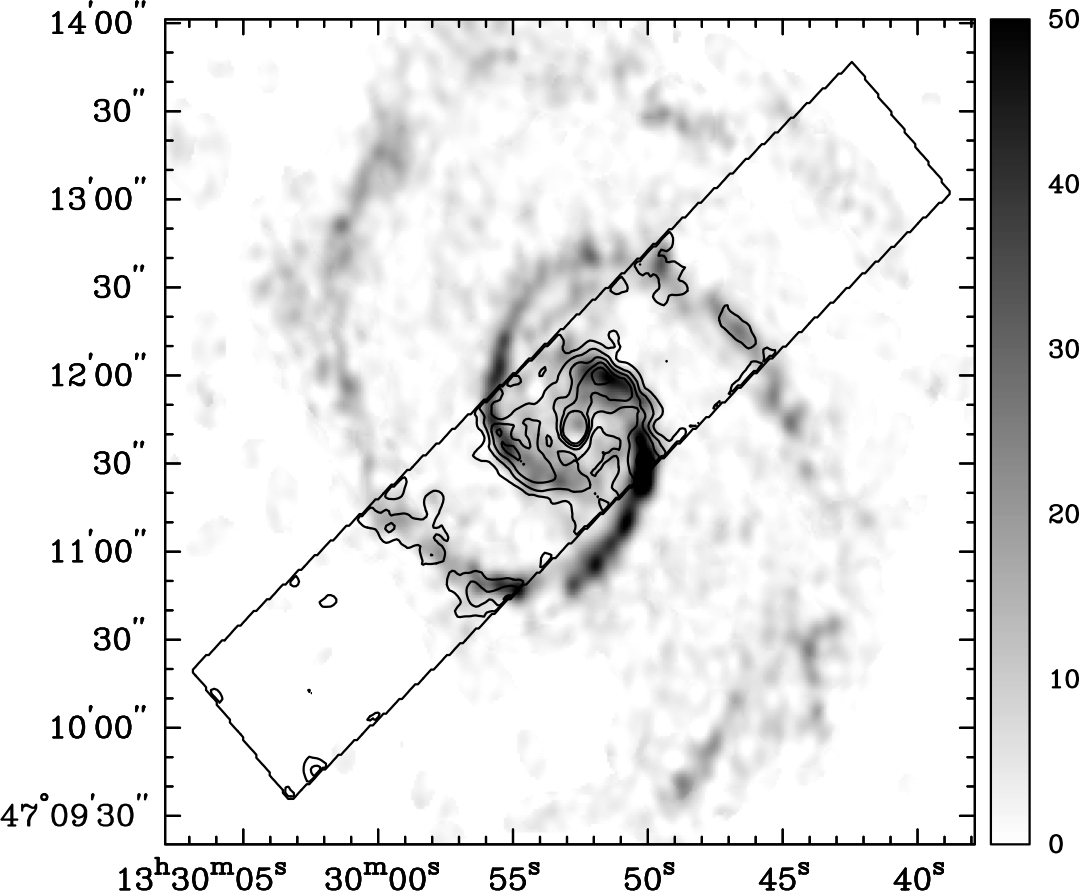
\includegraphics[width=8cm,angle=0]{bw_co_h2s2.jpg}
\hspace{0.1in}
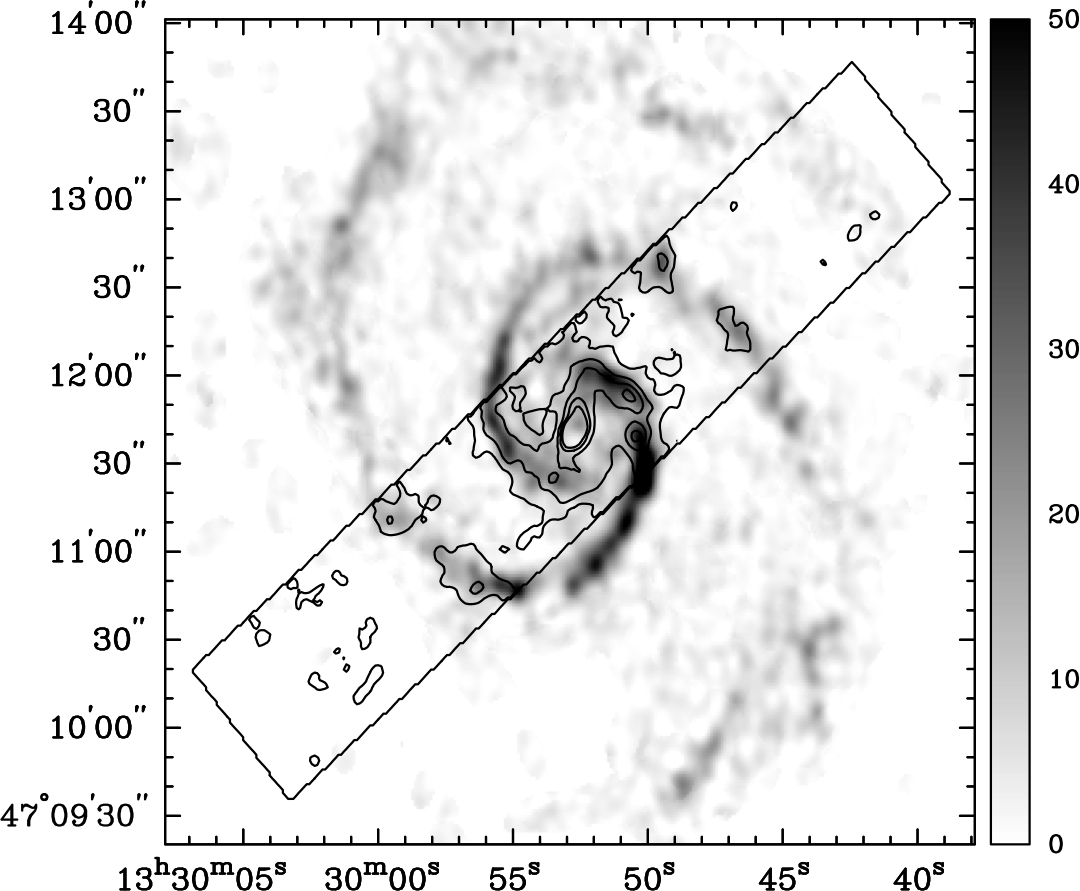
\includegraphics[width=8cm,angle=0]{bw_co_h2s3.jpg}}}
\caption{Comparison of the CO emission to the $\mathrm{H_2}$ S(0) ($top$ $left$),  $\mathrm{H_2}$ S(1) ($top$ $right$),  $\mathrm{H_2}$ S(2) ($bottom$ $left$),  and $\mathrm{H_2}$ S(3) ($bottom$ $right$) emission.  The CO emission maps are in units of Jy beam $\mathrm{s^{-1}}$.  Contour levels for $\mathrm{H_2}$ S(0), $\mathrm{H_2}$ S(1), $\mathrm{H_2}$ S(2), and $\mathrm{H_2}$ S(3) are the same as in Figure 1.\label{fig8}}
\end{figure}

\clearpage

%\begin{figure}[!h]
%\centerline{\hbox{\hspace{0.0in}
%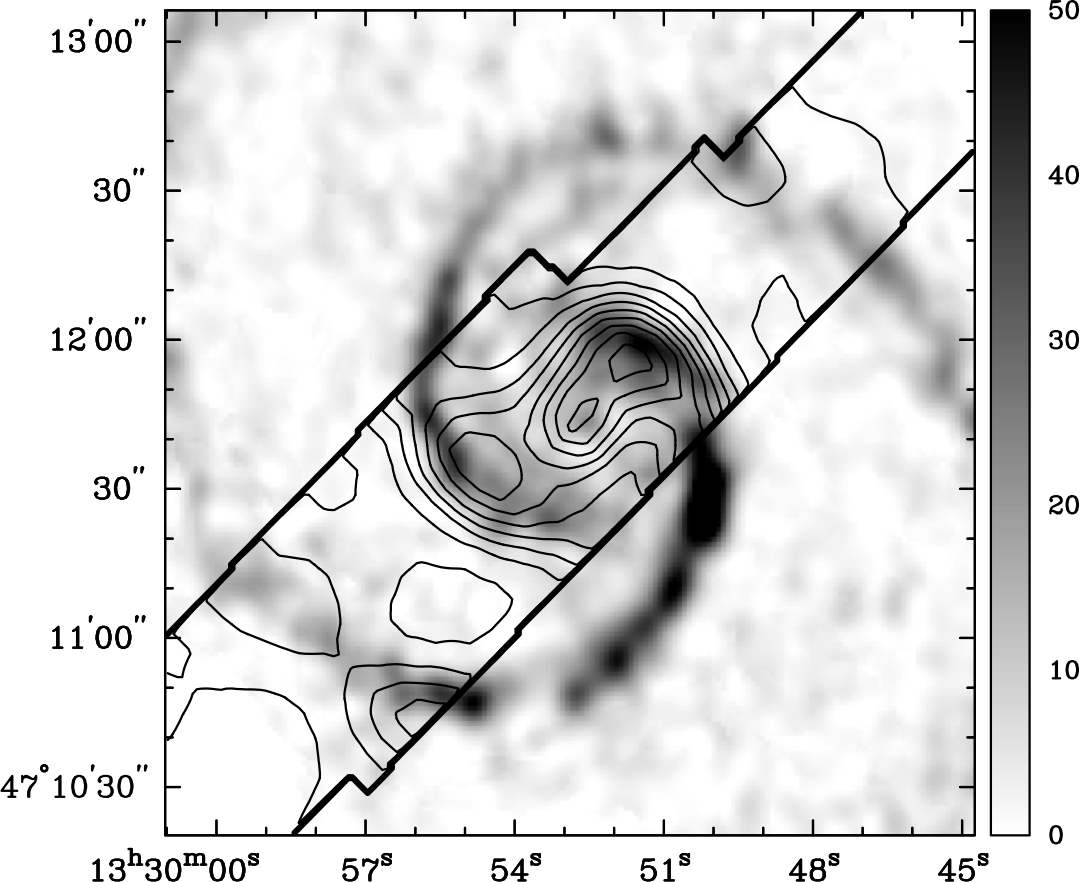
\includegraphics[width=8cm,angle=0]{bw_co_v_hot.jpg}}}
%\caption{Comparison of the cold $\mathrm{H_2}$ (as traced by CO emission) to the hot (T = 500-1000 K) %$\mathrm{H_2}$ mass.  Cold $\mathrm{H_2}$ mass is in units of $\mathrm{M_\sun}$. Hot $\mathrm{H_2}$ mass contours are the same as in Figure 5.\label{fig8}}
%\end{figure}

\begin{figure}[!h]
\centerline{\hbox{ \hspace{0.0in} 
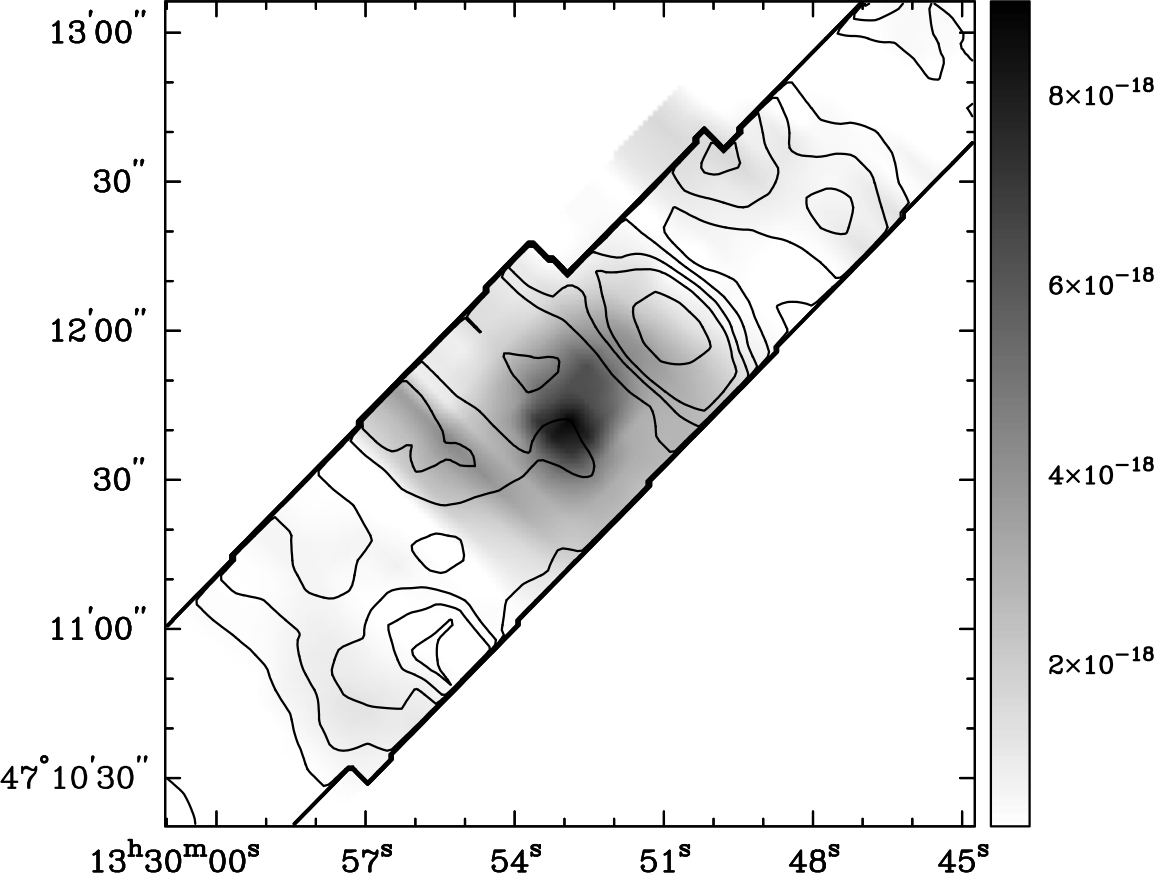
\includegraphics[width=8cm,angle=0]{oiv_v_warm_paper.jpg}
\hspace{0.1in}
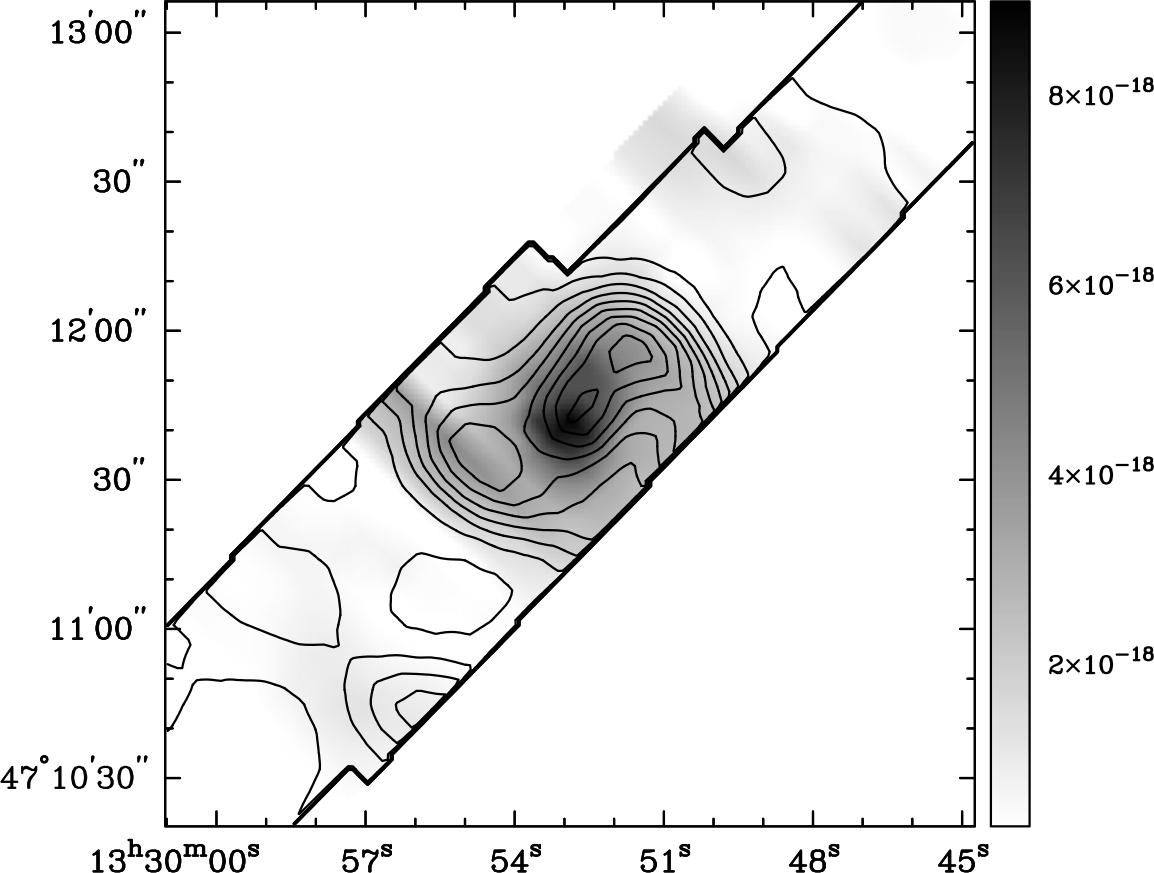
\includegraphics[width=8cm,angle=0]{oiv_v_hot_paper.jpg}}}
\caption{$Left$:  Comparison of the [O IV](25.89 \micron) emission (in grey-scale) to the warm (T = 100 K - 300 K) $\mathrm{H_2}$ mass distribution (in contours).  Hot $\mathrm{H_2}$ mass contours are the same as in Figures 3 and 4.  $Right$: Comparison of the [O IV](25.89 \micron) emission (in grey-scale) to the hot (T = 400 - 1000 K) $\mathrm{H_2}$ mass distribution (in contours).  Hot $\mathrm{H_2}$ mass contours are the same as in Figures 3 and 5.  The [O IV](25.89 \micron) emission is in units of W/$\mathrm{m^2}$.\label{fig9}}
\end{figure}

\clearpage

\begin{figure}[!t]
\centerline{\hbox{ \hspace{0.0in} 
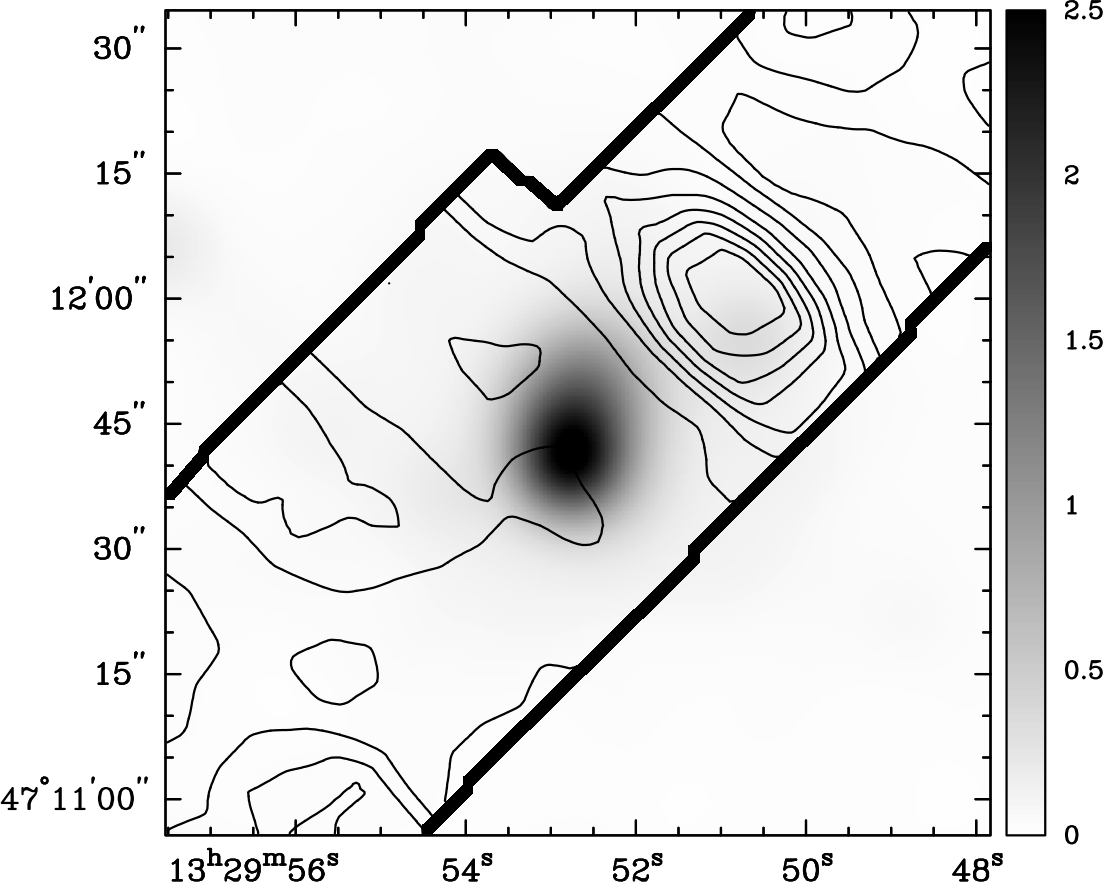
\includegraphics[width=8cm,angle=0]{x_v_cold.jpg}
\hspace{0.1in}
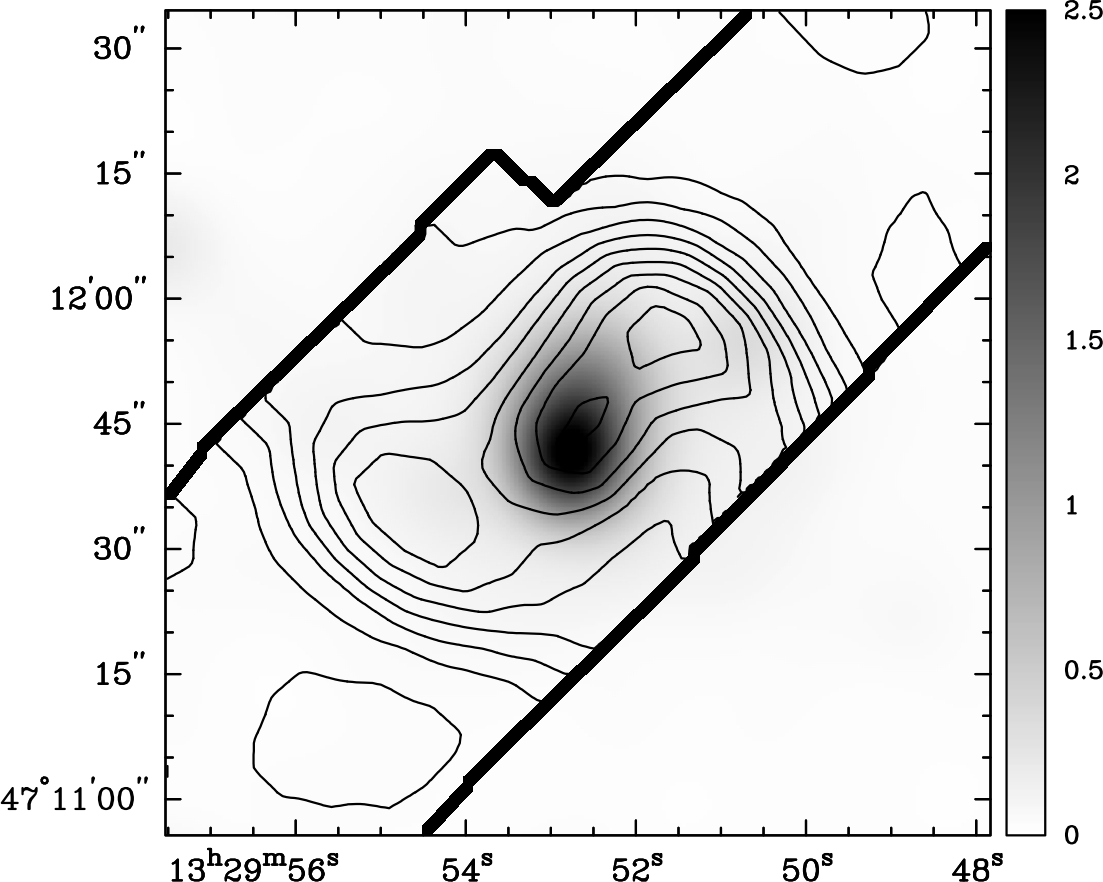
\includegraphics[width=8cm,angle=0]{x_v_warm.jpg}}}
\caption{$Left$:  Comparison of the smoothed 0.5 $-$ 10 keV X-ray emission band (in grey-scale) to the warm (T = 100 $-$ 300 K) $\mathrm{H_2}$ mass distribution (in contours).   The X-ray image has been smoothed to the same resolution as the warm $\mathrm{H_2}$ mass map.  X-ray emission is in units of counts.  $\mathrm{H_2}$ mass contours are the same as in Figures 3 and 4.  $Right$: Comparison of the smoothed 0.5 $-$ 10 keV X-ray emission band (in grey-scale) to the hot (T = 400 $-$ 1000 K) $\mathrm{H_2}$ mass distribution (in contours).  The $\mathrm{H_2}$ mass distribution contours are the same as in Figures 3 and 5.\label{fig10}}
\end{figure}

\clearpage

\begin{figure}[!h]
\centerline{\hbox{ \hspace{0.0in} 
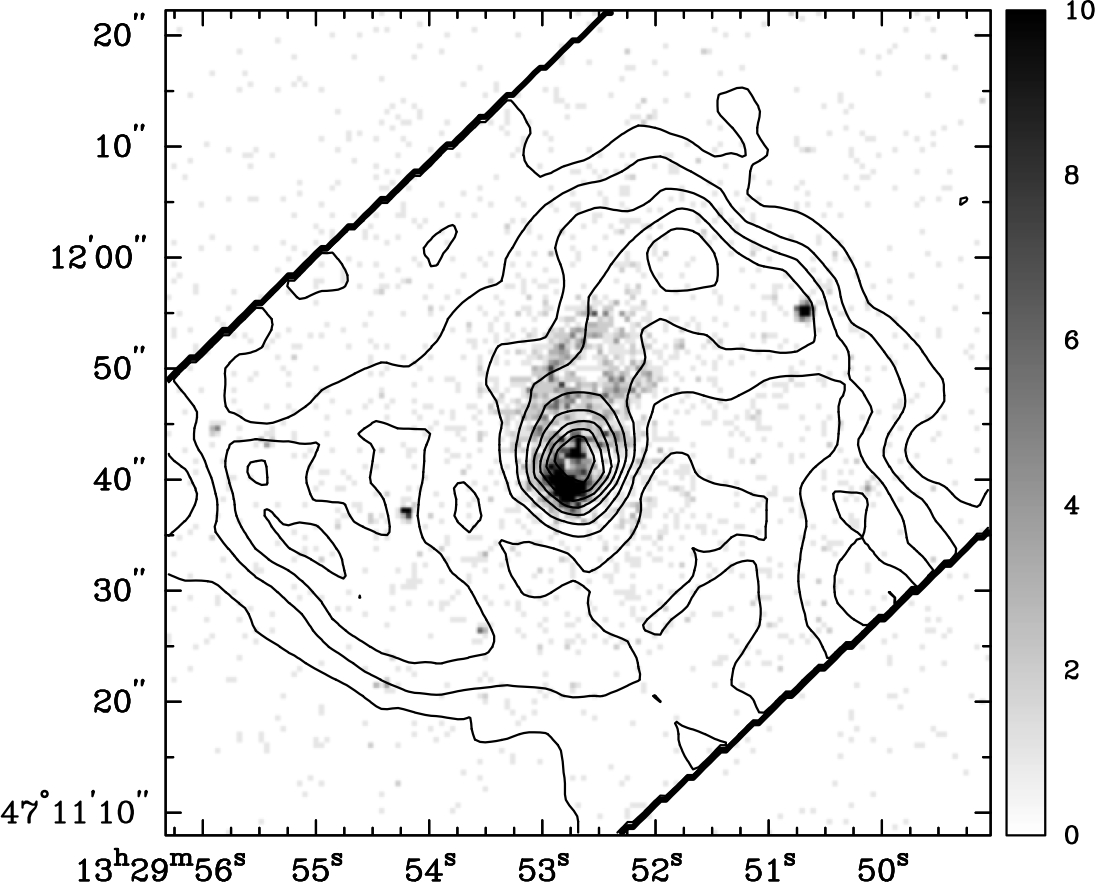
\includegraphics[width=8cm,angle=0]{bw_x_v_h2s2.jpg}
\hspace{0.1in}
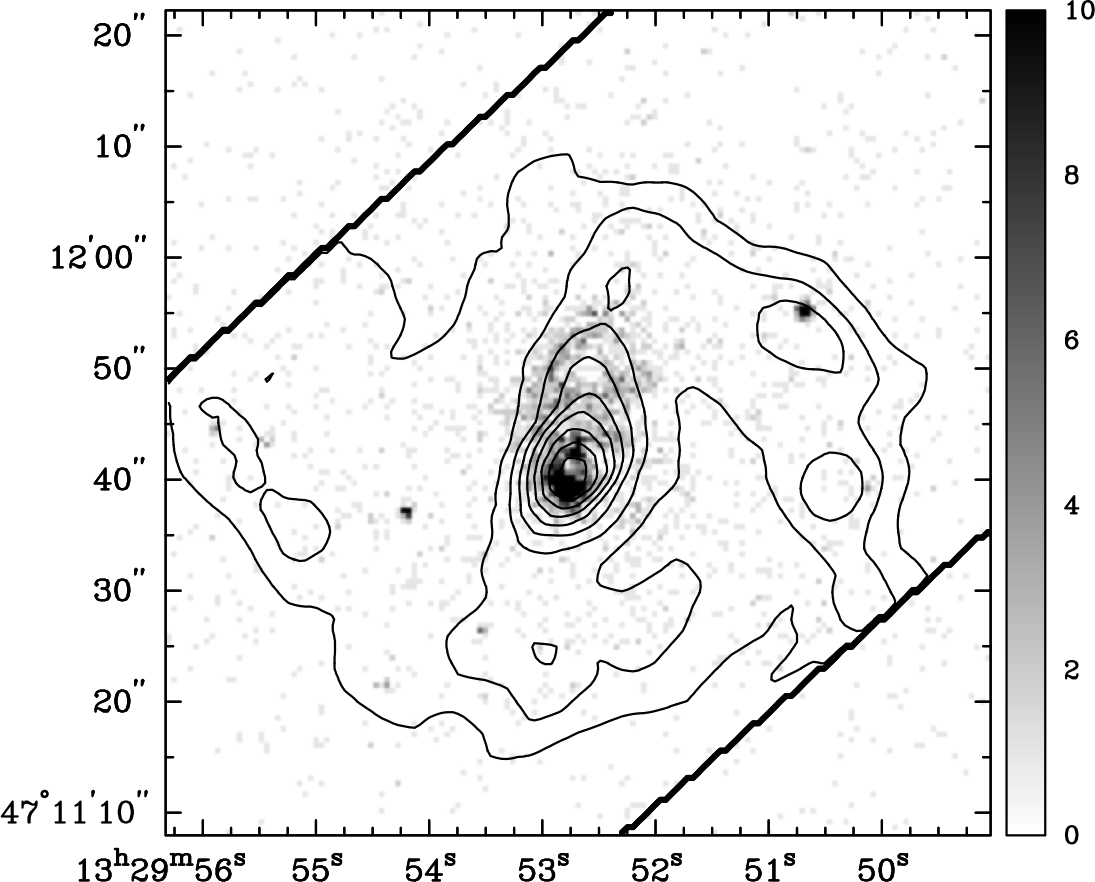
\includegraphics[width=8cm,angle=0]{bw_x_v_h2s3.jpg}}}
\end{figure}

\begin{figure}[!h]
\centerline{\hbox{\hspace{0.0in}
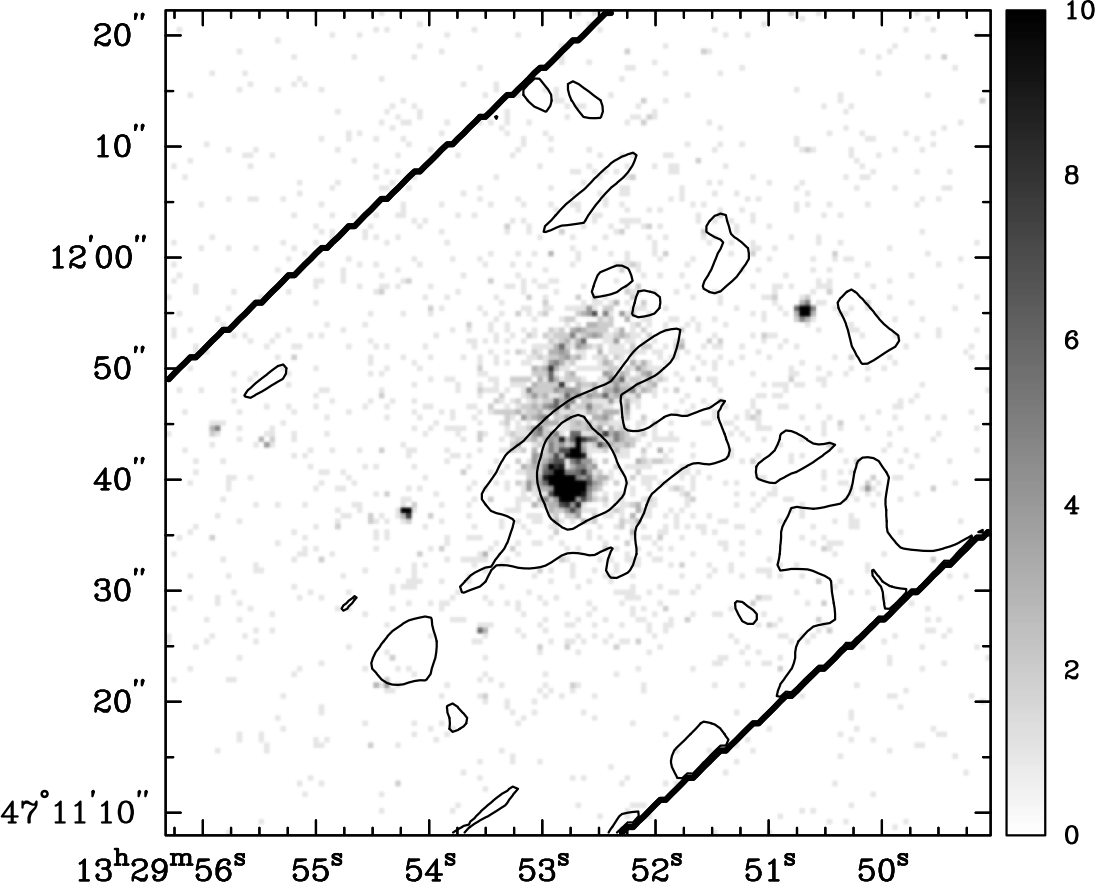
\includegraphics[width=8cm,angle=0]{bw_x_v_h2s4.jpg}
\hspace{0.1in}
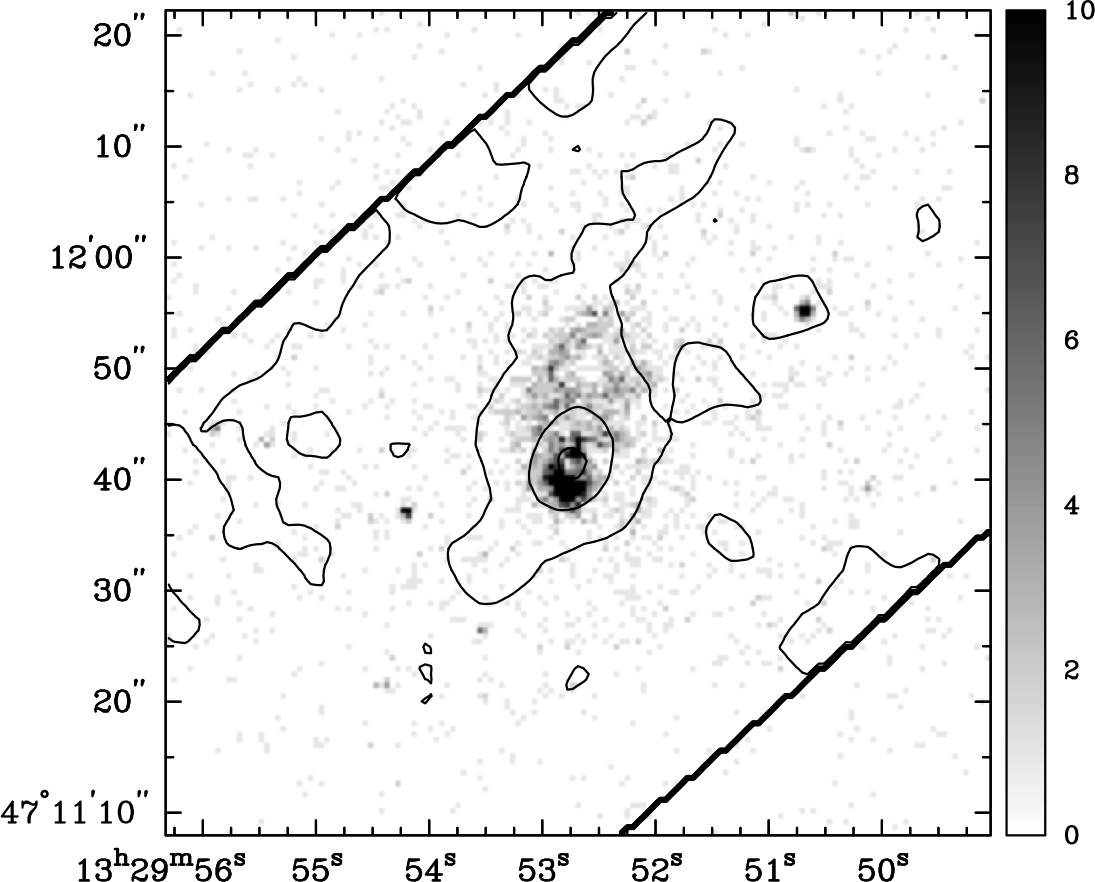
\includegraphics[width=8cm,angle=0]{bw_x_v_h2s5.jpg}}}
\caption{Comparison of the 0.5 $-$ 10 keV X-ray emission band (in grey-scale) to the $\mathrm{H_2}$ S(2) ($top$ $left$), $\mathrm{H_2}$ S(3) ($top$ $right$), $\mathrm{H_2}$ S(4) ($bottom$ $left$), and $\mathrm{H_2}$ S(5) ($bottom$ $right$) emission in the nuclear region of M51.  X-ray emission is in units of counts.  The $\mathrm{H_2}$ S(2) and $\mathrm{H_2}$ S(3) emission contours are at 10 \% of their peak values (2.20 $\times$ ${10^{-18}}$ and 1.35 $\times$ ${10^{-17}}$ W/$\mathrm{m^2}$, respectively).  The $\mathrm{H_2}$ S(4) contours are at  2.0 $\times$ ${10^{-18}}$ and 1.0 $\times$ ${10^{-18}}$ W/$\mathrm{m^2}$ and the $\mathrm{H_2}$ S(5) contours are at 7.3 $\times$ ${10^{-18}}$, 4.0 $\times$ ${10^{-18}}$, and 8.0 $\times$ ${10^{-19}}$ W/$\mathrm{m^2}$.\label{fig11}}
\end{figure}


\clearpage

%\begin{deluxetable}{cccccc}
%\tabletypesize{\scriptsize}
%\rotate
%\tablecaption{Resolution of the $\mathrm{H_2}$ Maps\label{tbl-2}}
%\tablewidth{0pt}
%\tablehead{
%\colhead{Transition} & \colhead{Wavelength (\micron)} & \colhead{Spatial Resolution} & \colhead{\lambda/\delta\lambda}
%}
%\startdata
%$\mathrm{H_2}$(0-0)S(0) & 28.22 & 10$\farcs$2 & 155  \\
%$\mathrm{H_2}$(0-0)S(1) & 17.04 & 6$\farcs$17 & 185 \\
%$\mathrm{H_2}$(0-0)S(2) & 12.28 & 4$\farcs$37 & 198 \\
%$\mathrm{H_2}$(0-0)S(3) & 9.66 & 3$\farcs$44 & 156 \\
%$\mathrm{H_2}$(0-0)S(4) & 8.03 & 2$\farcs$85 & 129 \\
%$\mathrm{H_2}$(0-0)S(5) & 6.91 & 2$\farcs$46 & 223 \\
%\enddata
%\tablecomments{Table lists the resolution of the $\mathrm{H_2}$ lines for which the extinction corrected flux has been mapped across the strip over \objectname{NGC 5194}.} 
%\end{deluxetable}


%\clearpage


\begin{deluxetable}{cccccc}
\tabletypesize{\scriptsize}
\rotate
\tablecaption{$\mathrm{H_2}$ Parameters %and Resolution of the $\mathrm{H_2}$ Maps
\label{tbl-1}}
\tablewidth{0pt}
\tablehead{
\colhead{Transition} & \colhead{Wavelength (\micron)} & \colhead{Rotational State (J)} & \colhead{Energy (E/k)} & \colhead{A ($\mathrm{s^{-1}})} & \colhead{Statistical Weight (g)} %& \colhead{Spatial Resolution} & \colhead{\lambda/\delta\lambda}
}
\startdata
$\mathrm{H_2}$(0-0)S(0) & 28.22 & 2 & 510 & 2.94$\times$${10^{-11}}$ & 5 \\ %& 10$\farcs$2 & 155 \\
$\mathrm{H_2}$(0-0)S(1) & 17.04 & 3 & 1015 & 4.76$\times$${10^{-10}}$ & 21 \\ % & 6$\farcs$17 & 185 \\
$\mathrm{H_2}$(0-0)S(2) & 12.28 & 4 & 1682 & 2.76$\times$${10^{-9}}$ & 9 \\ %& 4$\farcs$37 & 198 \\
$\mathrm{H_2}$(0-0)S(3) & 9.66 & 5 & 2504 & 9.84$\times$${10^{-9}}$ & 33 \\ %& 3$\farcs$44 & 156 \\
$\mathrm{H_2}$(0-0)S(4) & 8.03 & 6 & 3474 & 2.64$\times$${10^{-8}}$ & 13 \\ %& 2$\farcs$85 & 129 \\
$\mathrm{H_2}$(0-0)S(5) & 6.91 & 7 & 4586 & 5.88$\times$${10^{-8}}$ & 45 \\ % & 2$\farcs$46 & 223 \\
%$\mathrm{H_2}$(0-0)S(6) & 6.11 & 8 & 5829 & 1.14$\times$${10^{-7}}$ & 17 \\
%$\mathrm{H_2}$(0-0)S(7) & 5.51 & 9 & 7197 & 2.00$\times$${10^{-7}}$ & 57 \\
\enddata
\tablecomments{The statistical weight (g) is (2$J$ +1)(2$I$+1) where $I$ equals 1 for odd J transitions (ortho transitions) and $I$ equals 0 for even J transitions (para transitions).} 
\end{deluxetable}



\end{document}

